%%%%%%%%%%%%%%%%%%%%%%%%%%%%%%%%%%%%%%%%%
% Journal Article
% LaTeX Template
% Version 1.3 (9/9/13)
%
% This template has been downloaded from:
% http://www.LaTeXTemplates.com
%
% Original author:
% Frits Wenneker (http://www.howtotex.com)
%
% License:
% CC BY-NC-SA 3.0 (http://creativecommons.org/licenses/by-nc-sa/3.0/)
%
%%%%%%%%%%%%%%%%%%%%%%%%%%%%%%%%%%%%%%%%%

%----------------------------------------------------------------------------------------
%	PACKAGES AND OTHER DOCUMENT CONFIGURATIONS
%----------------------------------------------------------------------------------------

\documentclass[twoside]{article}

\usepackage{lipsum} % Package to generate dummy text throughout this template

\usepackage[sc]{mathpazo} % Use the Palatino font
\usepackage[T1]{fontenc} % Use 8-bit encoding that has 256 glyphs
\linespread{1.05} % Line spacing - Palatino needs more space between lines
\usepackage{microtype} % Slightly tweak font spacing for aesthetics

\usepackage[a4paper, top=32mm,bottom=32mm, left=35mm,right=35mm,columnsep=20pt]{geometry} % Document margins
\usepackage{multicol} % Used for the two-column layout of the document
\usepackage[hang, small,labelfont=bf,up,textfont=it,up]{caption} % Custom captions under/above floats in tables or figures
\usepackage{booktabs} % Horizontal rules in tables
\usepackage{float} % Required for tables and figures in the multi-column environment - they need to be placed in specific locations with the [H] (e.g. \begin{table}[H])
\usepackage{hyperref} % For hyperlinks in the PDF

\usepackage{lettrine} % The lettrine is the first enlarged letter at the beginning of the text
\usepackage{paralist} % Used for the compactitem environment which makes bullet points with less space between them

\usepackage{abstract} % Allows abstract customization
\renewcommand{\abstractnamefont}{\normalfont\bfseries} % Set the "Abstract" text to bold
\renewcommand{\abstracttextfont}{\normalfont\small\itshape} % Set the abstract itself to small italic text
%\newcommand{\P}{PRIMARQ}

\usepackage{titlesec} % Allows customization of titles
%\renewcommand\thesection{\Roman{section}} % Roman numerals for the sections
%\renewcommand\thesubsection{\Roman{subsection}} % Roman numerals for subsections
\titleformat{\section}[block]{\large\scshape\centering}{\thesection.}{1em}{} % Change the look of the section titles
\titleformat{\subsection}[block]{\large}{\thesubsection.}{1em}{} % Change the look of the section titles
\usepackage{enumerate}
\usepackage{graphicx}


\usepackage{fancyhdr} % Headers and footers
\pagestyle{fancy} % All pages have headers and footers
\fancyhead{} % Blank out the default header
\fancyfoot{} % Blank out the default footer
\fancyhead[C]{EUR Financial Mathematics $\bullet$ Fall 2013 $\bullet$ Budapest Semesters in Mathematics} % Custom header text
\fancyfoot[RO,LE]{\thepage} % Custom footer text

\usepackage{listings}
\usepackage{color}
\definecolor{dkgreen}{rgb}{0,0.6,0}
\definecolor{gray}{rgb}{0.5,0.5,0.5}
\definecolor{mauve}{rgb}{0.58,0,0.82}

\lstset{%frame=tb,
	  language=Python,
%	  aboveskip=3mm,
%	  belowskip=3mm,
	  showstringspaces=false,
%	  columns=flexible,
	  basicstyle={\ttfamily},
%	  numbers=none,
%	  numberstyle=\tiny\color{gray},
	  keywordstyle=\color{blue},
	  commentstyle=\color{dkgreen},
	  stringstyle=\color{mauve},
%	  breaklines=true,
%	  breakatwhitespace=true
%	  tabsize=3
}

%----------------------------------------------------------------------------------------
%	TITLE SECTION
%----------------------------------------------------------------------------------------

\title{\vspace{-15mm}\fontsize{24pt}{10pt}\selectfont\textbf{Investigations in Home Equity Position Markets}} % Article title

\author{
\large
\textsc{Dan Baron, Emily Searle-White}%\thanks{A thank you or further information}
\\[2mm] % Your name
\normalsize Western Washington University, Mills College \\ % Your institution
\normalsize {d.c.baron@gmail.com, esearlewhite@gmail.com} % Your email address
%\href{mailto:john@smith.com}
\vspace{-5mm}
}
\date{}

%----------------------------------------------------------------------------------------
%	MATH MACROS
%----------------------------------------------------------------------------------------
\usepackage{amsmath}

\newcommand\newc\newcommand
\newc\dt{\mathrm{d}t}
\newc{\E}{\mathbb{E}}
%\newenvironment{Dan}[0]{
	\renewcommand{\P}{\mathbb{P}}
	\newc{\V}{V_{\mathrm{now}}}
	\newc{\intdt}[1]{\int_0^\infty#1\ \dt}
	\newc\ali[1]{\begin{align*}#1\end{align*}}
%	}{}

\usepackage{color}
\newcommand{\hilight}[1]{\colorbox{yellow}{#1}}

\begin{document}

\maketitle % Insert title

\thispagestyle{fancy} % All pages have headers and footers

%----------------------------------------------------------------------------------------
%	ABSTRACT
%----------------------------------------------------------------------------------------

\begin{abstract}

\noindent Description here. %\lipsum[1] % Dummy abstract text

\end{abstract}

%----------------------------------------------------------------------------------------
%	ARTICLE CONTENTS
%----------------------------------------------------------------------------------------

%\begin{multicols}{2} % Two-column layout throughout the main article text

\tableofcontents
\pagebreak

\section{Introduction}

%As participants in the Budapest Semesters in Mathematics program in Fall 2013, Emily proposed an Elective Undergraduate Research project based on an internship during the preceeding summer. The internship was with a startup company called PRIMARQ in San Francisco.

In response to an internship with a company that hoped to create a market for the trade of equity positions in owner-occupied, residential real estate, Emily Searle-White suggested a research project to delve into the behavior of such a market. As such a market has never existed before and will differ from the known stock and real estate markets, 
%Emily hoped to model the growth and behavior of such a market and Dan offered to work with her in this research.

In the next few pages, we will present the structure of the overall market we are trying to model, the methods and techniques we used in specific aspects of the model, and our results. We will conclude with open questions and aspects to be explored further in the next iterations of the model.
%------------------------------------------------

\section{Structure of the Market}
To begin, we would like to present the overall structure of a transaction, as that forms the basis of the our model.  In broad terms, the model will track the creation and behavior of Home Equity Positions (hereafter referred to as HEPs). These HEPS are created as a portions of the equity in a home and sold to interested investors. These HEPs are later traded on the Secondary Market in the manner of normal stocks. The life cycle of a HEP can be briefly explained as follows:

\begin{enumerate}
\item{A homeowner triggers the creation of a HEP.}
\item{The new HEP, purchased for \$10,000, is auctioned to the lowest (in equity percentage) bidder among the investors. The equity percentage is now fixed for the life of the HEP.}
\item{The investor owning the HEP decides to sell the position and makes the HEP available on the secondary market.}
\item{The secondary market auction takes place, the HEP is sold to the highest (in dollars) bidder.}
\item{Repeat steps 3, 4.}
\item{The homeowner sells the underlying property and the HEP claim is said to mature.}
\item{The investor(s) is (are) paid the final claim value $C_f = S_f - M_0$ ($S_f$: the final sale price of the home; $M_0$ the initial mortgage amount). We use $M_0$ because the homeowner is reimbursed all principal payments from the sale proceeds before the remainder is divided between the homeowner and the investor.}
\end{enumerate}

We will explain in detail with an example. Homebuyer A decides to buy a home in San Francisco but asks PRIMARQ for an additional \$10,000 to help with the down payment, in exchange for a percentage stake in the equity of the home. Homebuyer A decides that she is willing to offer 8\% of the equity in her home in exchange for the \$10,000. So, she decides to offer this equity on the Exchange. 

Prospective investors registered with PRIMARQ have access to the Exchange website. There, they see that there is a position available in a home in San Francisco, that Homebuyer A is asking for the fixed \$10,000 and that she is opening the equity position bidding at 8\%. The investors also see some financial information about Homebuyer A, including her credit score, etc. The investors evaluate this position (including the home in question, the neighborhood and city in which is it located, etc) and investors B, C, and D decide to place bids to purchase the HEP.

Following their decisions to place a bid, investor B begins the process. He offers Homeowner A the \$10,000 in exchange for the 8\% equity position, as she originally offered. Investor C, thinking that the home will probably increase considerably in value in the next few years, offers to give Homebuyer A the \$10,000 but for only a 7.5\% position in the equity of the home. Investor D is more hopeful still and offers the \$10,000 for only a 7\% equity stake in Homebuyer A's new home. Investors B and C do not want to bid any lower, and Homebuyer A likes Investor D's offer, so Homebuyer A and Investor D enter into the transaction together. The equity percentage  of 7\% is now fixed for the entire lifetime of the HEP.

Homebuyer (now Homeowner) A and Investor D now own the home as Tenants in Common\footnote{Note: This is different in legal structure than a Joint Tenancy, specifically because Joint Tenancy includes Right of Survivorship, wherein upon the death of Homeowner A, the ownership of the home would pass to Investor D. This is \textit{not} the case in a Tenancy in Common. (US Department of Housing and Urban Development)}, and this arrangement will continue until one of two things happens: either Homeowner A decides to sell the home, or Investor D decides to sell his equity position\footnote{Specifically, the home is put in the name of the Homeowner and a Trust as Tenants In Common, and he beneficiary of that Trust is (are) the investor(s). In this manner, if the investors trade their positions, this does not affect the homeowner's claim to the home or the percentage in the equity split. The beneficiary of the fixed trust simply changes, which prevents the equity split having to be reevaluated with every sale of the HEP on he secondary market. For full details of the legal structure of a PRIMARQ transaction, see www.primarq.com.}. 

As soon as a home equity position has been created in a home, it can be sold and traded as a stock\footnote{We note here that normal equities of a company are all identical, whereas on the Secondary Market in this model, HEPs from the same home are identical but not HEPs from different homes.} on PRIMARQ's Secondary Market. If Investor D decides he wishes to sell his HEP, he can post his asking price on the Exchange for other registered investors to see. The HEP can change hands without any change happenening to the homeowner's claim to the home. The amount of equity assigned to a HEP does not change when the position is sold - the price may fluctuate as its market value changes (depending on the valuation of investors), but the underlying claim to the house remains fixed at the percentage assigned at the time of the HEP's creation.

If the homeowner decides to sell the home, then after all closing costs are paid and the homeowner is reimbursed for all prinicpal mortgage payments, the remaining profit is divided according to the originally decided equity split between the homeowner and whoever owns the HEP at the time, and the HEP position is terminated. If the new owner of the home decides to create a new HEP, then the process begins again.  

We now make a note of a few important rules in these transactions:
\begin{compactitem}
\item {More than one HEP can be in place in one home. This means that the homeowner may be on the title of the home with the Trust, and the Trust may have multiple benficiaries.}
\item The homeowner must always own the majority (51\%) of the equity in the home.
\end{compactitem}

This is the market that PRIMARQ is on its way to creating. Our job this semester was to try and see how this market might develop, using the research that has already gone in to modeling traditional equity and real estate markets. We broke the above process down and examined it away from the lense of a business model. Instead, we scrutinized each section of the transaction and tried to figure out which areas of mathematics would help us most in determining the behavior of such a theoretical market. 

\section{Our Approach}

We began by reviewing topics in Stochastic Calculus, which is an area frequently used in the analysis of financial markets. In particular, our study of Brownian Motions and other stochastic processes helped us to model the growth of a home's value in relation to the neighborhood around it. 

We also spent a good deal of time discussing Portfolio Theory, which is a branch of financial mathematics that deals with the behavior of risk and return when it comes to different bundles (or portfolios) of assets. As most of the investors in this model will have portfolios of their own, we wanted to make sure we had an understanding of the effects portfolio strategy and analysis can have on investor behavior, in particular the correlations between real estate related assets and the other asset classes . Further information on these topics can be found in Baxter and Rennie's \textit{Financial Calculus: An Introduction to Derivative Pricing} [1996] and also in Hull's \textit{Options, Futures, and Other Derivatives} [2009].

Finally, we reveiwed some literature on Prospect Theory, which is at the intersection of financial mathematics, behavioral economics, and psychology. Prospect Theory seeks to come up with models that fit the anomalies in the decision-making process that investors exhibit, leading to (what was traditionally considered as) irrational behavior. Again, as investors are a key part of the model we sought to build, we thought it vital to have at least a ground level understanding of the current research in investor behavior. We used Kahneman and Tversky's \textit{Prospect Theory: An Analysis of Decision Under Risk} [1979] for our main research on this topic.


\section{The Model}
Several areas of this model proved quite challenging. The modeling of the primary and secondary markets required an in-depth understanding of auctions. In addition to figuring out when and how much investors would bid on HEPs, it was also necessary to have an understanding of the behavior of the underlying neighborhoods in which the homes were located. Finally, if it is clear how a home is appreciating, how would an individual investor (with his or her own risk tolerance, etc.) evaluate that property? In addition, once a HEP is created, it is a financial instrument with an unmarked expiration date, with its own appreciation and depreciation according to the times. Understanding and tracking these aspects were the tasks that required the most attention.

\subsection{Structure and Implementation}
%\section{The Model}
%Our model was built up in several layers. The very ground layer was the structure of the neighborhoods in question. We wanted to model specifically five cities(San Francisco, Los Angeles, San Diego, Washington, DC and New York City)\footnote{These cities are based on the decided-upon launch cities for the company PRIMARQ.} and seven active\footnote{As time passes in the model, more neighborhoods become active, depending on the average HEP value in the rest of the city and other factors.} neighborhoods within each of these cities. Within each neighbohood, there were a certain number of HEPs available at the start. The number of homes available grows within the model depending on how each neighborhood is appreciating, along with other factors that might spark investor interest. 
to do.

\subsection{Challenges}

\subsubsection{Expectation}\label{subsubsec:expectation}
%\subsection{Expectation}
%\begin{Dan}
Let the random variable $T$ be the time at which some HEP expires, i.e., at which the underlying house is sold. Let the random variables $S_T$ and $V$, respectively, be the sale price of the home and the final payout value of the HEP. We thus have $V=p(S_T-M_0)$, where $p$ is the HEP claim percentage. Recall that $M_0$ refers to the initial mortgage amount.


The expectation of the present value $\V$ of $V$, given that the HEP expires at some particular time $t$, is just 
$$
	\E[\V\mid T=t] = \left(\E[S_t]-M_0\right)e^{-rt},
$$
where $r$ is the discount rate. But of course the home could be sold at any time in the future (or never). If $f$ is the probability density function of the distribution of $T$, then we must have
	\ali{
	\E[\V] = \intdt{f(t)\left(\E[S_t]-M_0\right)e^{-rt}}.
	}

In this model, we assume that $T$ is exponentially distributed, with the parameter $\lambda$ derived from census data. The expectation of the home sale price is trickier; the neighborhood appreciation is log-normal, but the value of an individual home depends on the aging constant and a series of discrete price changes as well as this appreciation.

Our solution was to assume that the appreciation $S_T/s_0$ can be well approximated as a random process of the same form as the neighborhood appreciation process; i.e.,
$$
S_t\approx s_0\exp\left({\int_{0}^{t}\sigma_*\mathrm{d}W_s + \int_0^t\mu_*\mathrm{d}s}\right)\quad(t\geq0),
$$
where $\mu_*$ equals the log-mean of the neighborhood appreciation (after all, a neighborhood is just a bunch of houses) but $\sigma_* ^2$ is larger than the neighborhood log-variance.

Upon the introduction of a new ``neighborhood'' object, the HEP market model generates a large random sample of appreciation ratios $s_1/s_0$ from our home value model and records the log-mean and log-variance of this sample, $\mu_*$ and $\sigma_*^2$. With these numbers and the assumptions mentioned above, we have $\E[S_t]\approx \exp\left({\mu_*t+\sigma_*^2t/2}\right)$ and hence
\ali{
	\E[\V] 
		&=
	\intdt{f(t)\left(\E[S_t]-M_0\right)e^{-rt}}
		\\&
	\approx 	\intdt{\lambda e^{-\lambda t-rt}\left(s_0e^{\mu_*t+\sigma_*^2t/2}-M_0\right)}.
		}
Provided that $\mu_*+\sigma_*^2/2-\lambda-r<0$, this converges to
$$
\frac{\lambda s_0}{-\mu_*-\sigma_*^2/2+\lambda+r}+\frac{\lambda M_0}{-\lambda-r}.
$$

To handle the divergent case, we regard the discount rate $r$ as the best available risk-adjusted return in the larger financial universe. If the inequality above does not hold, then in fact there is a better return available -- namely, on investment in real estate in this neighborhood. We adjust the parameter $r$ accordingly.
%\end{Dan}

\subsubsection{Evolution of Home Prices}
%\subsection{Evolution of Home Prices}%\begin{Dan}
We assume that the appreciation $A=m_1/m_0$ of the median home price $m_t$ in any neighborhood in one year is log-normally distributed, with some log-mean $\mu$ and log-variance $\sigma^2$.

However, the evolution of an individual property's price might diverge wildly from the evolution of median prices in the neighborhood. In the absence of any previous literature on the topic, we modeled the price evolution process as the interaction of three distinct, simpler processes: the neighborhood appreciation, a constant depreciation rate, and discrete jumps in price. The first of these we have already discussed.

The depreciation rate reflects general wear and tear as the home ages. We set a depreciation constant $\alpha$ and use the product $s_1=(1-\alpha)s_0$ to model this process.

But the homeowner will not sit idly by while the home falls to pieces. Major repairs and home improvement projects such as new bathrooms or roofs are all modeled by discrete price jumps. Fires, floods, and other disasters are also considered here.

The American Housing Survey\footnote{US Census Bureau, American Housing Survey} data includes the proportion, $p$, of respondents who undertook at least one home improvement project in the two years since the previous survey. Assuming that the number of such events in a particular house, $N$, is $\mathrm{Pois}(\lambda)$, we can conclude that
$$
\P\left(N\geq1\right)=p\implies \lambda = -\frac{1}{2}\log\left(1-p\right)\frac{_\text{\tiny{events}}}{^\text{\tiny{year}}}.
$$

An initial challenge in this research was finding an appropriate mean value for these discrete price jumps. In our earliest tests, the median of the home appreciation ratios generated by the model would never match the neighborhood appreciation rate. But of course the price of every house in the neighborhood is imagined to evolve according to this process, and so they must match.

If $J=\{J_1, J_2, \dots, J_N\}$ are the values of the discrete jumps that occur in one year and $A$ is the neighborhood appreciation ratio in that year, then our home price process is given by
$$
\frac{S_1}{ s_0}=\frac{A(1-\alpha)(1+\sum_{k=1}^NJ_k)s_0}{s_0}.
$$
We then use this formula to find the correct expectation for discrete jump values. If $A$ and $S_1/A$ are assumed to be independent, then we have
$$
\E\left[\frac{S_1}{ s_0}\right]=\E\left[\frac{A(1-\alpha)(1+\sum_{k=1}^N)s_0}{s_0}\right] = \E[A](1-\alpha)\left(1+\E\left[\sum_{k=1}^NJ_k\right]\right).
 $$ 
But $\E[S_1/s_0]=\E[A]$, and this equation reduces to
$$
\E\left[\sum_{k=1}^NJ_k\right]=\frac{1}{1-\alpha}-1.
$$
We model $J$ as an I.I.D. normal random sample, with sample mean \newcommand{\Jbar}{\overline{J}}$\Jbar$, and we have
\ali{
\E\left[\sum_{k=1}^NJ_k\right]&=\E\left[N\Jbar\right]
\\&=\E\left[N\right]\E\left[\Jbar\right]
\\&=\lambda\E\left[\Jbar\right]
}
The correct expectation for discrete jump values is therefore $\frac{\alpha}{\lambda(1-\alpha)}$.

%egraphics[scale=.39]{sigmaWmuTcopy.pdf}

\hilight{Some of the assumptions mentioned here may be problematic; this may be an area for further refinement.}\\

%\textbf{Example}\\

\begin{figure}

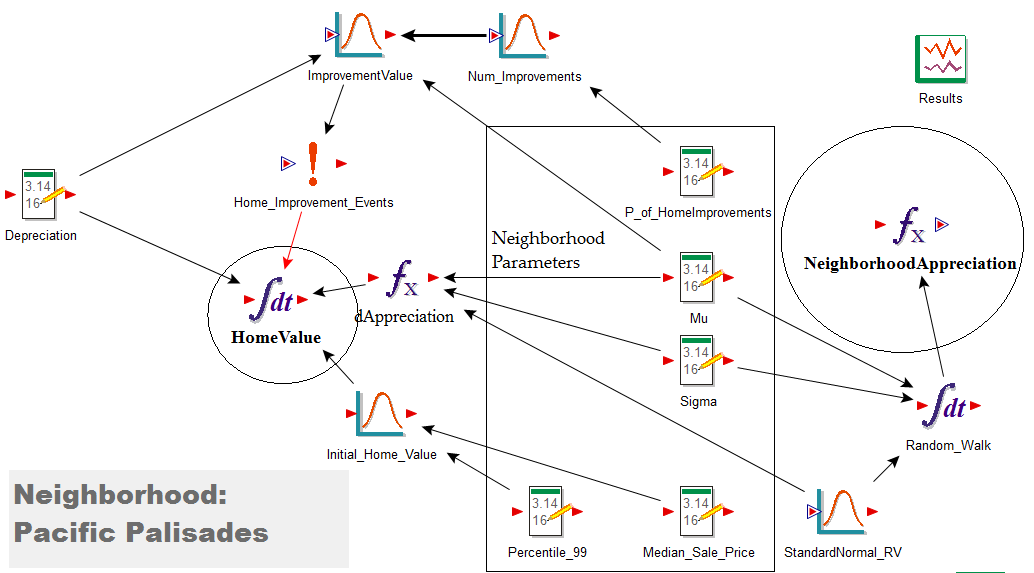
\includegraphics[scale=.35]{GoldSimScreenshot3.png}
\caption{Basic Neighborhood Appreciation Model in Goldsim\copyright}
\end{figure}

%The above picture shows how we visualized the process of a home valuation originally in the GoldSim\copyright\footnote{Copyright 2013 GoldSim Technology Group.}  model. 

%\includegraphics[scale=.39]{Home.pdf}

%\end{Dan}
\subsubsection{Investor Valuation}
Financial instrument pricing theory is a well-researched field, but results often contradict one another and investors often seem to ignore the theory altogether. Generation of investor valuations for each HEP was therefore one of the more challenging aspects of this project.

We began by considering the expectation of the present value of the payout of a HEP at the time of its expiration, as discussed in \ref{subsubsec:expectation}. While useful, this does not reflect investor attitudes about risk. We therefore turned to Prospect Theory as a source of concrete valuations.

Prospect Theory suggests that human perceptions of probability and of the value of wealth outcomes are somewhat skewed. In particular, if a risky prospect has value $x$ with probability $p$ and value $y$ with probability $(1-p)$, then an individual investor will consider the prospect to be worth
\ali{
u=w(p)v(x)+w(1-p)v(y),
}
where $v$ and $w$ are weighting functions. Gonzalez and Wu discuss the family of probability weighting functions given by
$$
w(p) = \frac{p^\beta}{\left(p^\beta+(1-p)^\beta\right)^{1/\beta}}\quad(0<\beta\leq1);
$$
we include their chart here. We used this family of functions for each investor's $w$, with uniformly distributed parameters $\beta$.

\begin{figure}
\centering
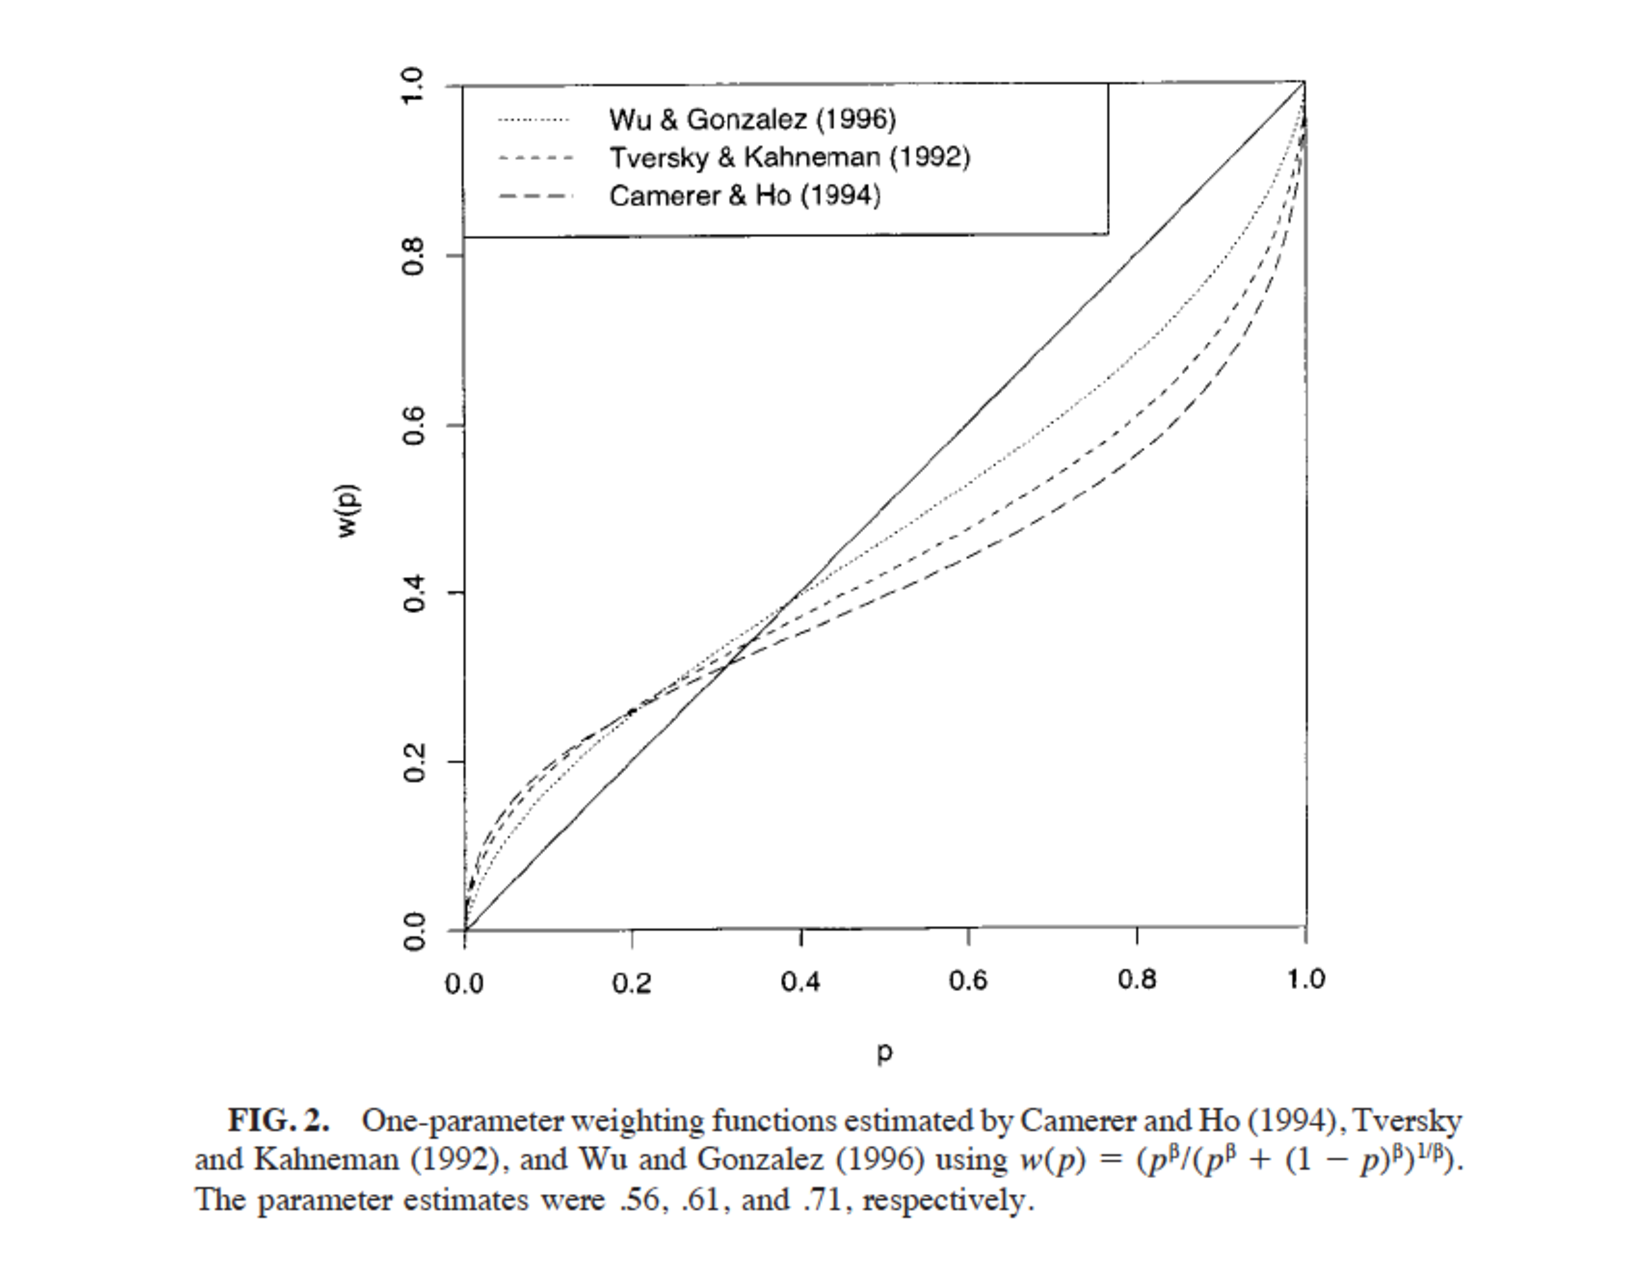
\includegraphics[width=.65\linewidth]{WeightingFunction.pdf}
\caption{Weighting Function}
\end{figure}

Each investor's $v$ function has the form 
$$v(x)=\begin{cases}
\gamma_1\log(\frac{x}{\gamma_1}+1)&\text{if }x\geq 0\\
-\gamma_1\gamma_2\log(\frac{-x}{\gamma_1}+1)&\text{if }x< 0.
\end{cases}
$$
The parameter $\gamma_1$  measures the investor's risk tolerance; as $\gamma_1\to\infty$, $v(x)$ approaches the line with slope 1. Prospect theory also suggests that losses hurt more than gains feel good, and the parameter $\gamma_2$ measures this effect.\

\begin{figure}[H]
\caption{Prospect Theory?}
\centering
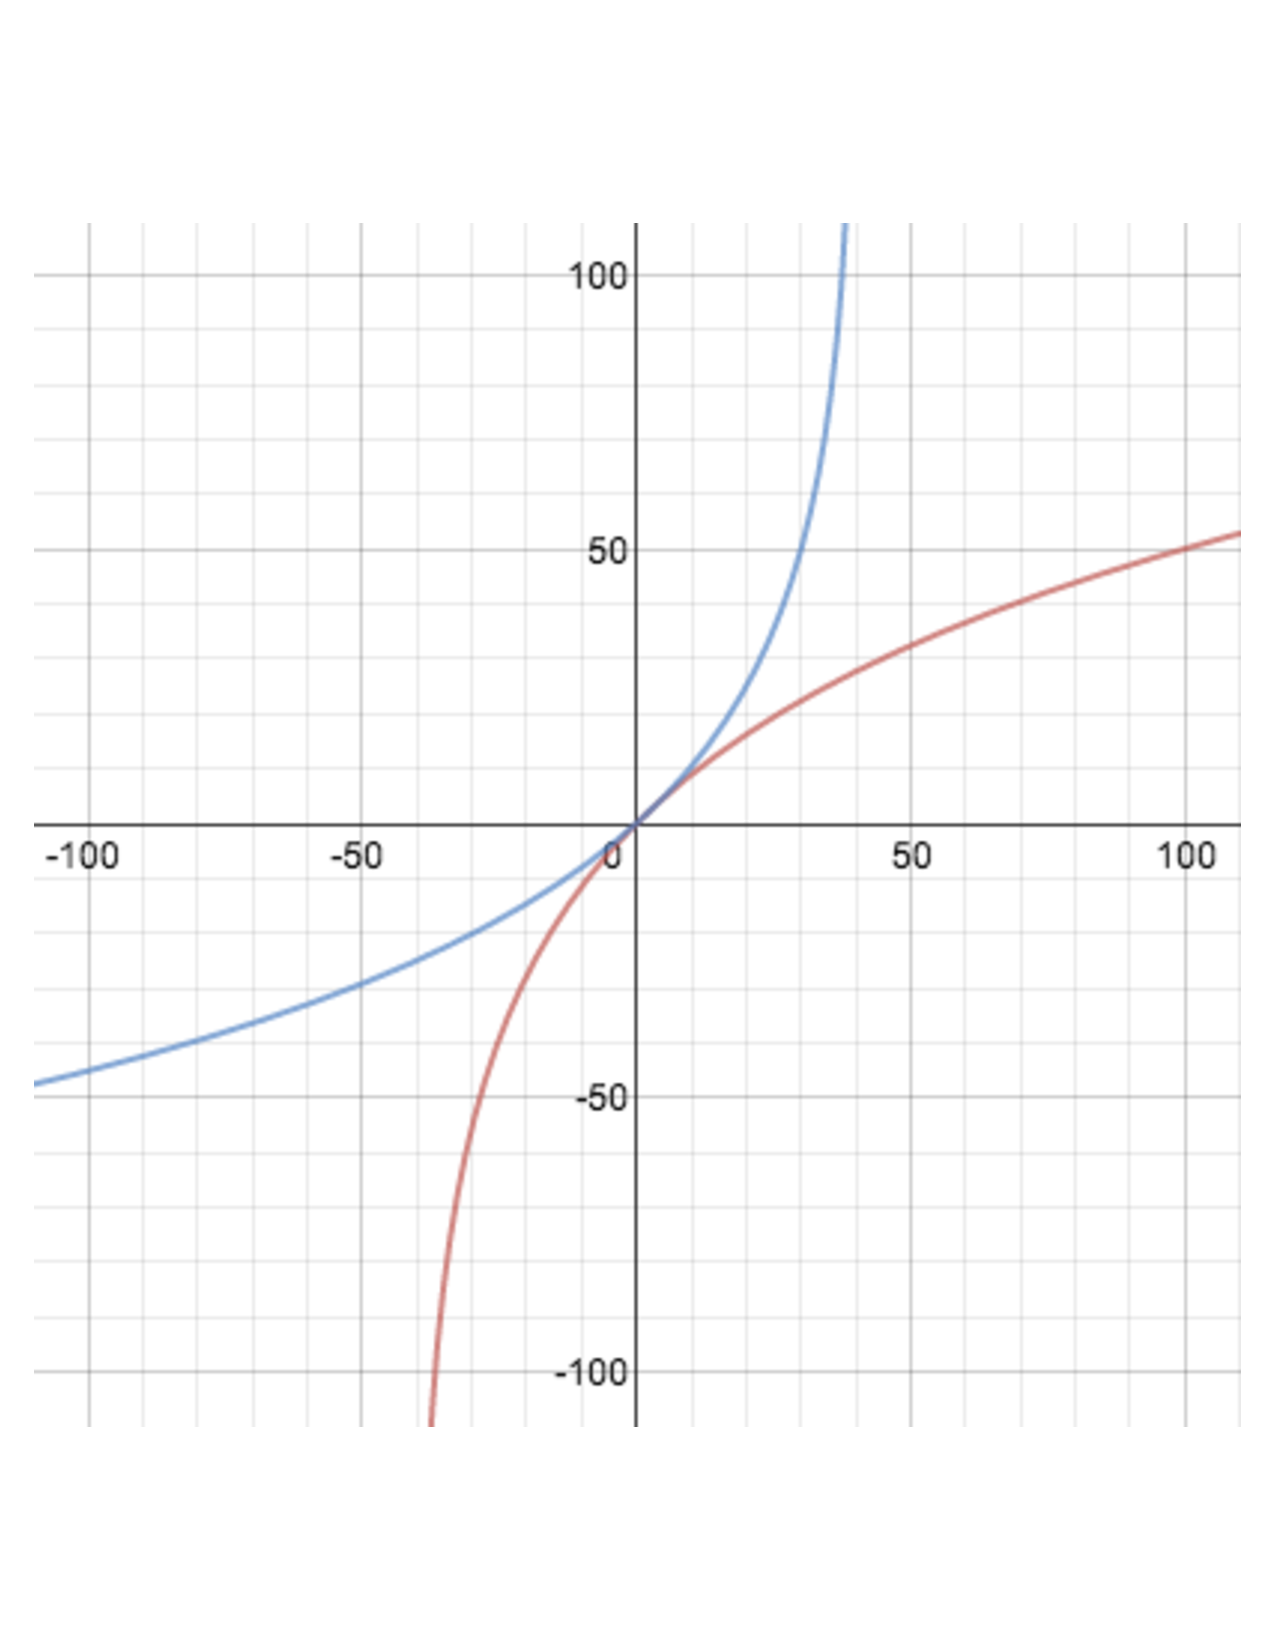
\includegraphics[scale=.39]{FlipFlop.pdf}
\end{figure}

We use these functions to compute each investor's valuation on a HEP, but we must first understand the distribution of $\V$, the discounted eventual payout. For each neighborhood object, our HEP market model generates a (realization of a) large random sample of pairs $(T,S_T/s_0)$ from our home price evolution model, where $T$ is the exponentially distributed waiting time until the home is sold and $S_T$ is the final sale price.

The appreciation $S_{t_\beta}/s_{t_\alpha}$ after any interval of length $t_\beta-t_\alpha$ is identically distributed for all homes that share a neighborhood. We therefore record the complete random sample discussed in the preceding paragraph and use it each time we need to approximate the cumulative distribution function of $\V$ for some HEP with claim percentage $p$. The value of the underlying real property changes with each timestep in the model, but if $s_{\alpha}$ is the value at time $t_\alpha$ and $(t,s_t/s_0)$ is a datum from the random sample, then 
$$
v_\mathrm{now} = p\left(\frac{s_t}{s_0}s_{\alpha}-M_0\right)
$$
is a realization of $\V$.

After constructing the approximate CDF $F(x)=\P(\V<x)$, we obtain each investor's valuation on the HEP. In the original cumulative prospect theory paper, Tversky and Kahneman give this as
$$
U=\int_{-\infty}^0 v(x)\left(\frac{d}{dx}w(F(x))\right)\,dx-\int_0^{+\infty} v(x)\left(\frac{d}{dx}w(1-F(x)\right)\,dx.
$$
Our model is limited to a discrete approximation of $F$, so we employ the finite Riemann sum 
\ali{
U&=\sum_{k=1}^{m} v(F_{.01k})\left(w\left(.01k\right)-w\left(.01k-.01\right)\right)\\&\phantom{=}-\sum_{k=m+1}^{100} v(F_{.01k})\left(w\left(1-.01k\right)-w\left(1.01-.01k\right)\right),
}
where $F_{.01k}$ is the $k$th percentile of $F$ and $m\%=F(0)$.

Later iterations of this market model will employ additional techniques for generating investor valuations, but the process described here has already yielded interesting results.


\subsubsection{Auctions: Primary and Secondary Markets}
Our algorithm simulates home equity position auctions in the following manner.

We gather from each investor object a valuation on the real property underlying the HEP--or rather, on a hypothetical 100\% claim on the equity of that property. The investor's bid is then proportional to the HEP claim percentage in the case of secondary market auctions, and is given by $(\$10,000/\mathrm{Valuation})$ in primary auctions. 

A "bid" in this program and a bid on the Primarq
 marketplace are not quite the same entity.
 Here, the variable \verb+bid.value+ is the best that an investor
 would be willing to bid; she will not actually bid
 so much unless forced up in a "bidding war" with
 another investor, and then only if she has the necessary cash at hand.

 The \verb+winner+ and \verb+secondbid+ attributes of an
 auction instance track the two best bids in the
 above sense. After creating a bid for each investor, \verb+winner.value+
 is adjusted to be only slightly better than \verb+secondbid.value+.
Our algorithm is an abstraction of a day's bidding, during which each investor may have placed several actual bids or even none.

 What we are technically modeling is therefore an iterated
 second-price sealed-bid auction, or iterated Vickrey auction. In both Vickrey auctions and  the more familiar English auctions, the price paid is the second-highest valuation. The dominant strategy is identical in both types of auction as well: bid your full valuation. 
 
 The Vickrey auction's sealed bids usually prevent the mechanism of price discovery, by which bidders' valuations influence one another. This effect is important in English auctions (the actual auction type in place in the HEP market), so we incorporate it by iterating the Vickrey auction, opening the bids at the end of each iteration. To our knowledge, this is the first paper to investigate iterated Vickrey auctions.

The choice of the iterated Vickrey auction for this model was motivated by simplicity and computational efficiency; we did not wish to model each investor's bidding frequency, attention span, time zone, or other such trivialities. However, this choice introduced a new challenge: with several auctions potentially running in parallel and resolved simultaneously, the algorithm must ensure  that no bidder wins more auctions than she can afford.

The present implementation handles this recursively. We simulate one Vickrey iteration for each ongoing auction and record each bidder's winning bids. These are then sorted in descending order of preference; i.e., by how well the investor likes the price she will end up paying. From the beginning of the list, each auction that an investor has won and can afford is considered finished for the day.

Upon reaching an auction in the list that the investor has won but cannot afford (because she spent her money on the auctions she liked better, earlier in the list), it is assumed that the investor never actually placed that bid. The remainder of the list is sent back to be run again. This time, everyone's available bidding cash will have been adjusted down to reflect the auctions that they definitely won.
%Within each neighborhood, the given homes each have a certain value, determined by several factors. These factors include the home's depreciation due to age, the neighborhood appreciation, and the value added or subtracted by home improvement projects and disasters, respectively. The picture below depicts one neighborhood in Los Angeles: Pacific Palisades. Here, neighborhood-specific data is used to calculate the average home value, neighborhood appreciation, etc. Every home in each neighborhood will have is value calculated in such a way.




%------------------------------------------------



%------------------------------------------------

\section{Results}
Here we see the results of the auction in the primary market. The simulation was set up for one home in one neighborhood, with ten investors ( where the individual risk tolerance is a fixed function of the portfolio wealth of that investor) on the market. Here we have an example of the bidding process on a new HEP in the Primary Market:

\begin{figure}[h!]
  \centering
      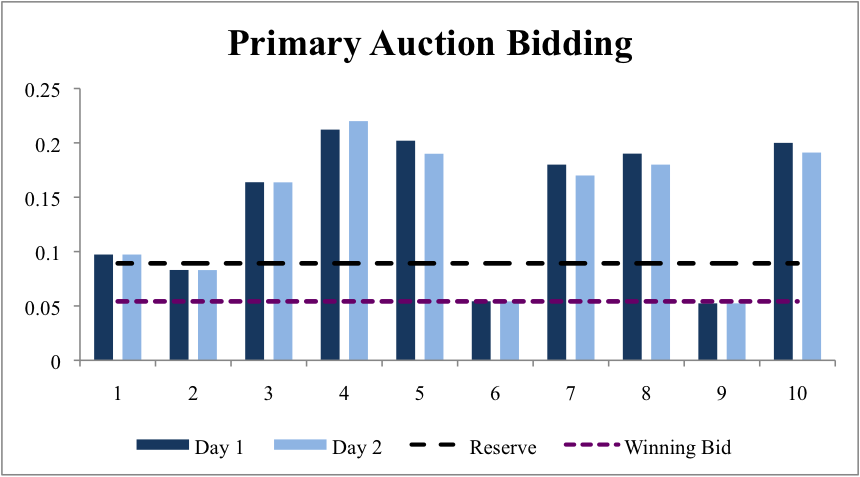
\includegraphics[scale=.7]{PrimaryAuction.png}
  \caption{The investors are numbered on the X-Axis. Their percentage bids are represented in columns. The HEP in question was sold after two days, so two bids are shown (one for each day) from each investor.}
\end{figure}

The percentage claim on the equity of the home is fixed at the time of creation of a HEP. However, through the appreciation of the neighborhood and hence the home, as well as through investor interest, the HEP's value can grow independently of the home. Further, even though the claim value is a fixed percentage, say at 10\%, even at the time of its creation, the HEP's value (\$ 10,000 at the start) in relation to the overall equity in the home may be far more (or less) than that 10\%. We watched this relationship through one hundred realizations of one HEP being sold once after ten years.

In addition, for another hundred realizations (monitored every thirty days), we monitored the relationship between the expectation of the HEP in a home and the home's value over that time. The resulting data indicates an important aspect of the HEP: the HEP is a leveraged financial product. Because there is always a mortgage on the home in question, the appreciation on the home results in extreme appreciation on the equity in proportion. The chart below shows the evolution over five years of the ratio between a HEP's expectation and the current home value. Both are
\begin{figure}
\centering
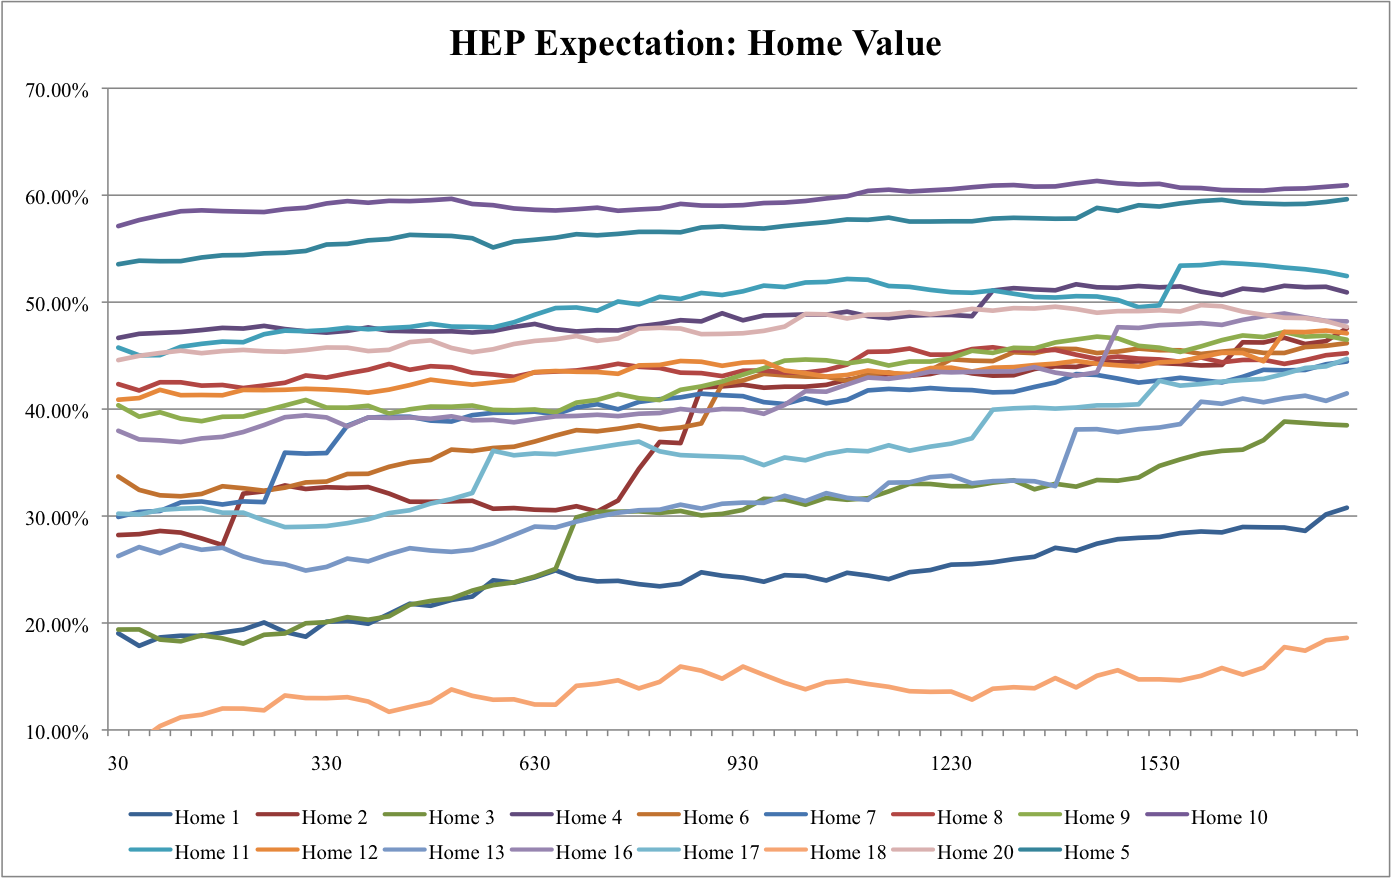
\includegraphics[scale=.55]{HepExpHVal.png}
\caption{Expectation of HEPS of 17 Homes in Relation to the Overall Home Value}
\end{figure}
%    \begin{tabular}{|lccc|}
%    \hline
%    HEP & Percentage Claim & Original P-E Ratio & New P-E Ratio \\ \hline
%    HEP 1 & 11\% & 8.95 \% & 10.31\% \\
%    HEP 2 & 16.9\% & 29.37\% & 30.93\%\\
%    HEP 3 & 19.1\% & 39.4\% & 45.1\% \\
%    HEP 4 & 8.2\% & 7.22\% & 9.38\% \\
%    HEP 5 & 8.5\% & 59.05\% & 54.92\% \\
%    HEP 6 & 19.7\% & 53.42\% & 24.93\% \\
%    HEP 7 & 11.6\% & 10.28\% & 6.75\% \\ \hline
%    \end{tabular}
%\end{table}


%------------------------------------------------

\section{Discussion: Next Steps}
There are several aspects of the model that, as we progressed, found were too complex to tackle completely in one semester. Many of these things could either be simulated randomly for the first iteration of the model, or could be simply put on hold until a later version. 
% what kinds of results can we look at in the future? Parameter sets, bubbles, etc. 

\subsection{Investor Behavior}
We hoped to use both Portfolio Theory and Prospect Theory to have a better understanding of investor behavior. However, as time grew to a close in the semester, we decided that modeling the auction process in the primary market and the trading in the secondary market was more important than having the complex investor profiles that we originally had planned. The model is structured in such a way that given more time, it will be easy to insert a more complex investor profile. As it stands, events like the timing of an investor's bid in the primary market are triggered by values chosen at random from a distribution. This and other similar situations in the model can be more accurately triggered if more of the information from Prospect Theory was built in.

In addition, given more time and communication with PRIMARQ, a more accurate idea of the registered investors portfolios, and thus a better view of how much they would be likely to invest in the HEP market. 

\subsection{Neighborhood Behavior}
Emily spent a great deal of time during her internship starting to model the process of neighborhood appreciation. As investors are most interested in investing in areas they believe will appreciate in the future, coming up with a predictive index for neighborhood appreciation is very valuable. Through the course of her time with PRIMARQ, she researched and discovered upwards of twenty different factors that influence the appreciation of a neighborhood. However, at the end of her internship, Emily was not finished with this index. More research is needed to complete the task, and the time required for that project wasn't available in addition to the time needed for the task at hand. So, as in the section above, Dan and Emily researched which kinds of distributions are used that most accurately reflect neighborhood appreciation and used that in the model for now. Given the time to finish this index, the research behind it would certainly be a useful aspect to add into the model, and as with the investor behavior, there is room for it to be encorporated.


%----------------------------------------------------------------------------------------
%	REFERENCE LIST
%----------------------------------------------------------------------------------------
\newpage

\section{Reviewed Works}
%{thebibliography}{99} % Bibliography - this is intentionally simple in this template
\begin{itemize}
\item{BAXTER M. / RENNIE A. Financial Calculus: An Introduction to Derivative Pricing. Cambridge, UK: Cambridge University Press. 1996.}
\item{GONZALEZ, R. / WU, G. "On the Shape of the Probability Weighting Function". Cognitive Psychology, 38(1999), pp. 129-166. }
\item{HULL, J. Options, Futures, and Other Derivatives. Upper Saddle River, NJ: Pearson Education, Inc. 2009.}
\item{KAHNEMAN, D. /  TVERSKY A. Prospect Theory: An Analysis of Decision Under Risk. Econometrica: Journal of the Econometric Society (1979). pp. 263-291.}
\item{MIKLOS, R. Prospect Theory and its Financial Applications. Universiteit van Amsterdam. 2011.}
\item{SHREVE, S. Stochastic Calculus for Finance II :Continuous-Time Models. Pittsburgh, PA. Springer. 2008.}
\item{United States Census Bureau. "AHS 2011 National Summary Report and Tables". \emph{American Housing Survey}. 2011 }
\item{VICKREY, W. Counterspeculation, Auctions, and Competitive Sealed Tenders. The Journal of Finance 16(1961). Columbia University.}
\end{itemize}

%\bibitem[Figueredo and Wolf, 2009]{Figueredo:2009dg}
%Figueredo, A.~J. and Wolf, P. S.~A. (2009).
%\newblock Assortative pairing and life history strategy - a cross-cultural
%  study.
%\newblock {\em Human Nature}, 20:317--330.
 
%\end{thebibliography}

%----------------------------------------------------------------------------------------

%\end{multicols}
\newpage

\section{Appendix}
\subsection{Notes About Software}
The choice of software was a complicated one for this project. For several reasons, the program GoldSim\copyright\ was optimal. Not only is the software designed for large model implementations (specifically using Monte Carlo simulations for things like Risk Analysis and Decision Analysis), but also Emily had had some experience with it over the summer. In addition, GoldSim\copyright\ is a very visual environment that can display results and show the model design in explanatory ways, and link dynamically with other programs for data (such as Excel).  Finally, there were several pieces of data that were available to Emily and Dan only via this software (from employees at PRIMARQ), and so the decision was made to use GoldSim\copyright\ as the primary software.

However, several difficulties arose. The first was that the modeling of HEP behavior in the market (tracking the speed of growth in value, tracking which owners own the HEP at what time, and for how long) is something that falls very easily into the object-oriented programming paradigm, which is not supported by GoldSim\copyright. Dan had a lot of experience in Python, Emily in Java, and working to overcome this block in GoldSim\copyright\ was often very discouraging.  In addition, the amount of calculations that GoldSim\copyright\ performs during the Monte Carlo simulation process proved to be just a bit too much data for our laptops to handle, at least at the level of complexity that we wanted it to work.

In the end, we decided it was best to plan our model conceptually in GoldSim\copyright\ (as it provides a nice, visual overview, with a clear picture of what elements depend on what in the model). We used that software as our drawing board, but build the bulk of the model in Python, and then used GoldSim\copyright 's many features to help display our results from the simulations.

For the next iteration of this project, we think use of GoldSim certainly could be helpful, but without the computer power necessary, we think the same issues would arise.

\subsection{Python Code}
%\begin{lstlisting}
##########################################################
##########################################################
###
### Welcome, one and all, to the world's first and only
###
###              Exceptionally Amazing
###           Home-Equity-Position-Market
###            Prognosticating Simulator!
###
### Brought to you by Daniel Baron and Emily Searle-White.
###
##########################################################
##########################################################   (#tag)


############################################
## Simulation settings
############################################
# to do: make output nice and easy. Interactive?
output= 'trackOne'
fieldNames = [
    'Time',
    'Home Value',
    # 'Waffles',    # If you don't need a particular item,
                    # just comment out the line -- DON'T DELETE!
    'Equity',
    'HEP Expectation'#,
    #'Investor Valuations',
    #'E.D.B.',       # Expectation-Derived-Bid; the correct auction
                    # bid if you only care about the expected value
                    # of the HEP.
    #'Investor Bids',
    #'Reserve',
    #'Best Bid',
    #'Winning Bidder' #, # Make sure there is no comma after the
                        # final entry in the list.
    ]

realizations = 100

# All time quantities are in years
duration = 5
# We want to adjust the time resolution within each simulation
# run to improve efficiency.
from fractions import Fraction
longTimeStep = Fraction(1,12)   # 30-day months and 360-day
shortTimeStep = Fraction(1,360) # years, for simplicity.



agingRate = 0.02 # annual depreciation due to aging

sim = True
HomeSalesOn=False
trackOne=True
stopAfterPrimary=False
stopAfterSecondary=False
numSources = 1
numInvestors=10
sellHep = 0#######  ########  ####

###########
#Neighborhood settings:

nbhdDict = dict(city = 'St Louis', # Geographic location
          AppreciationMean = 5, # Quoted in percentage points,
            # so that AppreciationMean = 5 implies 5% annualized
            # home appreciation.
          sdMultiplier = 0.8, # The geometric std deviation of
            # home appreciation is derived from AppreciationMean
            # and this multiplier, so that AppreciationMean = 5
            # and sdGeoMultiplier = 0.8 imply that a
            # (1 + 0.8) * 5% = 8%
            # return is one standard deviation above the mean.                
          medianPrice = 2.257 * 10**5, # Median home price
          percent99= 3, # 99th percentile of home prices,
            # expressed as a multiple of the median.
          pHIP= .52, #Percentage of households reporting at
            # least one Home improvement project in 2 years.
          pDisaster= NotImplemented, # Percentage of households
            # reporting at least one disaster repair project in
            # the 2 year reporting period.
          initialHomes = 3, # Homes seeking HEPs at t=0.
          spawnRate = 3 # New homes seeking HEPs per year
          )
if stopAfterPrimary or stopAfterSecondary or trackOne:
    nbhdDict['spawnRate']=0
    nbhdDict['initialHomes']=1
nbhdDicts = [nbhdDict]

auctionLength = 5*shortTimeStep #Controls when auctions stop.
    # Not yet implemented.


############################################
## Imports, Constants, and Utilities
############################################

from random import random, gauss, choice, \
     shuffle, lognormvariate, expovariate
from math import floor, ceil, log, exp, modf
from types import InstanceType
from csv import DictWriter as dictWriter, DictReader as dictReader
from os import chdir, mkdir
err = RuntimeError

gauss99 = 2.326347874 # 99th percentile
sellDateLambda = 1./13 * log(2) # Parameter of the exponential
  # distribution governing homeowner turnover.

from time import ctime as __now__
now = lambda: __now__().replace(':','..')

class Q(Fraction):
# Modification of Python's rational number class:
# automatically limits the denominator to reasonable values,
# and stringifies in mixed-number form for readability.
    def __new__(cls, numerator=0,denominator=None):
        X=Fraction(numerator,denominator)\
           .limit_denominator(1000)
        return X
    def __str__(self):
        if self.denominator == 1: return str(int(self))
        elif abs(self)<1:
            return str(self.numerator) + '/' \
                   + str(self.denominator)
        else:
            return str(int(self)) + ' ' \
                   + str( abs( self-int(self) ))

class dataClass:
# This is just a generic data wrapper.
    def __init__(self, **args):
        self.__dict__.update(args)

# Keeps track of how many of each object have been made so far.
index = dataClass(last={})

# The discount rate.
riskFree = dataClass(rate=log(1.03));
riskFree.Rate=riskFree.rate

# Auction length, not yet implemented #to do
auctionLength = dataClass(days=auctionLength)

def poissonvariate(lambd):
# Returns a Poisson-distributed random number.
    if lambd<0: raise ValueError, "The poisson parameter must"\
      "be nonnegative."
    lambd=float(lambd)
    k = 0
    p = random()
    
    # P(X = 0) and P(X <=0):
    P= exp(-lambd)
    cumP = P

    while p>cumP:
        k+=1
        P *= lambd/k    #P(X=k)
        cumP += P       #P(X<=k)
    return k

def mean_and_variance(iterable, corrected=False):
# Compute and return the mean and variance of a list
# of numbers.
    sumX = 0
    squareSumX = 0
    for i in iterable:
        sumX += i
        squareSumX += i**2

    try: n= float(len(iterable))
    except TypeError:
        n=0.
        for i in iterable:
            n += 1.
    mean = sumX/n
    
    if corrected: divisor = n-1.
    else: divisor = n
    variance = (squareSumX - n*mean**2)/divisor

    return {'mean':mean,'variance':variance}

##########
# Some logic functions.

__any__=any;__all__=all
def any(*args):
    try: return __any__(*args)
    except TypeError: return __any__(args)
def all(*args):
    try: return __all__(*args)
    except TypeError: return __all__(args)

none = lambda *args: not any(*args)
notAll = lambda *args: not all(*args)

def ifElse(condition, valueIfTrue, valueIfFalse=None):
    if condition:
        return valueIfTrue
    else:
        return valueIfFalse
##########

def randomWalk(mu,sigma,dt):  # For modified Brownian motion
    return gauss(mu*dt,sigma*dt**.5)

##########
# Output data to csv
output=dataClass(   name = output,
                    folder = output + '. ' + now(),
                    data = {},
                    isOn = 1#False
                    )
if output.isOn:
    mkdir(output.folder); chdir(output.folder)
del mkdir, chdir

def investorFields(field):
    if field in fieldNames:
        k = fieldNames.index(field)
        n = k + numInvestors
        j=0
        
        field = field.split(" ")[1][:-1] # assuming the plural just ends in 's'
        field = field + ' #'
        while k < n:
            j += 1; k += 1
            fieldNames.insert(k, field +str(j))

investorFields('Investor Valuations')
investorFields('Investor Bids')    

def makeOutput():
    with open(output.file,'ab') as f:
        writer = dictWriter(f,fieldNames, extrasaction='ignore')
        writer.writerow(output.data)
##        for key in output.data:           db
##            print key,output.data[key]   db

def prep_outFile():
    output.file = 'realization '+str(realization)+'.csv'
    output.data = dict((name,'') for name in fieldNames)
    headers = dict((name,name) for name in fieldNames)
    f=open(output.file, 'wb')
    
    writer = dictWriter(f,fieldNames, extrasaction='ignore')
    writer.writerow(headers)
    f.close()
#########
        
############################################
## Class Declarations
############################################
## Much of the implementation relies on classes and instances
## to represent the abstract "HEPs", "Investors", etc.
## Some of these are little more than data wrappers, but
## there are also big chunks of the simulation procedure coded 
## here as class methods.

class thingClass:
# The parent class; everybody else inherits these attributes
    
    def __str__(self):
    # Gives each Thing a name for it to print, eg "HEP 28".
    # To do: make it easy to print all relevant data,
    # e.g. "HEP 28-- House: 9, Claim: 2.1%, Owner: Bob."
        name = str(self.__class__).split('.')[1].split('lass')[0][:-1]
        name = name + " " + str(self.id)
        return name

    def copy(self):
    # Makes a shallow copy 
        copy = self.__class__(**self.__dict__) # Most have
          # initialization requirements.
        copy.__dict__.update(self.__dict__)
        return copy

    def __init__(self, **args):
    # Track how many Things of this class have been made,
    # give this new Thing an ID number.
        try:
            index.last[self.__class__] += 1
            self.id = index.last[self.__class__]
        except KeyError: # "self" is the first instance of class
            index.last[self.__class__]=self.id=1


class HEPclass(thingClass):
# The Home Equity Positions.

    def __init__(self,house,**args):
        # Each new-minted HEP has a house, but,
        # as yet, no owner, nor fixed percentage.
        thingClass.__init__(self) 
        self.needsPrimary=True
        self.needsSecondary=False
        self.atAuction=False
        self.owner=None
        self.house=house
        self.percentage=args.get(   # Initialize at 1,
            'percentage',           # except for testing
            args.get('p',1))        # purposes.
        house.heps.add(self)

    def getReservePrice(self):
    # The minimum price that a seller will accept at auction.
        if self.owner == None:
            return gauss(1, .05)*valu(self.house)
        else:
            return gauss(.95,.05)*self.owner.getValu(self.house)

    def expire(self):
    # When the underlying house is sold, remove this HEP from
    # the list and pay the investor.
        heps.remove(self)
        self.house.heps.remove(self)
        if self.owner != None:
            self.owner.liquidWealth += payout(self)
            self.owner.heps.remove(self)

    def transfer(self, newOwner, price=0):
    # Transfer the HEP to a new owner, usually as a result
    # of sale at auction.
        
        if self.owner != None:
            self.owner.heps.remove(self)
            self.owner.liquidWealth += price

        newOwner.heps.add(self)
        newOwner.liquidWealth  -= price
        self.owner = newOwner
        
hepClass = HEPclass


class neighborhoodClass(thingClass):
# Neighborhoods.

    def __init__(self, **args):
    # Function __init__ should receive keyword arguments corresponding
    # to the keys in the Neighborhood Settings dictionary discussed in
    # the Simulation Settings section. The easiest way to do this is
    # unpack such a dictionary in the invocation:
    #    neighborhoodInstance = neighborhoodClass(**neighborhoodDict)
        thingClass.__init__(self)

        # mu is the mean log-appreciation, e.g. log(1.05)
        self.mu = log( args["AppreciationMean"]*0.01 + 1 )
        args.pop("AppreciationMean")
        
        # sigma is the square root of the log-variance, given
        # as a multiplier on the mean annualized appreciation.
        self.sigma = log( (1-1/meanGeo)*args["sdMultiplier"]+1)
        args.pop("sdMultiplier")

        self.__dict__.update(args)
        self.appreciation={t:1}
        self.lastTime = t

        # Find the parameters of the Poisson processes
        # governing Home Improvement Projects and Disasters.
        self.lambda_HIP = -log(1-self.pHIP)*0.5
        self.lambda_Disaster = NotImplemented # to do
        #-log(1-self.pDisaster)*0.5

        # Keep track of the houses in this hood with live HEPs:
        self.houses = set()

        # Get the parameters for the log-normal distribution
        # from which we take initial home prices.
        self.priceMu = log(self.medianPrice)
        self.priceSigma = log(self.percent99)/gauss99
    
    def copy(self, t, tabulaRasa = True):
        copy = thingClass.copy(self)
        if tabulaRasa:
            copy.houses=set()
            copy.appreciation={t:1}
        return copy
            
    def appreciate(self, t):
    # Determine the appreciation ratio for the neighborhood
    # median home price since the last time we checked:
    # app(t,s) = app(s)*exp( mu*(t-s) + sigma*sqrt(t-s)*X ),
    # where t>s and X~N(0,1).

        # Have we gone back in time?
        if t< self.lastTime:
            
            #Scrub all traces of the alternate timeline.
            future = True
            time=self.appreciation.keys()
            time.sort()
            time.reverse()
            for Time in time:
                if Time > t : self.appreciation.pop(Time)
                elif future:
                    future = False
                    self.lastTime = Time
                    break                

        # Calculate the appreciation of the median home price since lastTime
        dt = t-self.lastTime
        dApp = exp(randomWalk(self.mu, self.sigma, dt))
        # Record the total appreciation since t=0.
        self.appreciation[t] =  dApp * \
                               self.appreciation[self.lastTime]

        #update all houses in this hood:
        for house in self.houses:
            house.updateValue(dApp, dt)

        self.lastTime = t
        
        #either update all houses whenever neighborhood is updated,
        # or update everybody only once per month,
        # or keep dictionary of appreciation values.

    def getInitialPrice(self):
    # I assume here that home prices are log-normally distributed;
    # thus the median price determines the mean, mu, of the log-prices,
    # and sigma is such that P( X < percent99*median) = 0.99:
    #
    #       self.priceMu = log(self.medianPrice),
    #       self.priceSigma = log(self.percent99)/gauss99. 
        return lognormvariate(              \
            self.priceMu, self.priceSigma)  \
            * self.appreciation[self.lastTime]

    def getInitialMortgage(self):
    # The median current mortgage debt in the US, as a percentage of the
    # value of the home, is 71%; a 100% mortgage is roughly the 80th
    # percentile value. Homeowners seeking HEPs will, in general, have better
    # than average credit, but will also often be assuming a new mortgage
    # on a newly purchased home -- a mortgage not yet payed down.
    #
    # I assume here that these two effects roughly cancel out, so that
    # the cumulative distribution of debt/value ratios is the same in
    # the HEP world as in the world at large; I further assume that the
    # ratios are log-normally distributed.
    #
        log_point71 = -0.342490309      # log(0.71)
        mortgage_sigma = 0.406941146    # -log(0.71)/z80
        return lognormvariate(log_point71, mortgage_sigma)

    def newHouses(self, t):
    # How many houses need new HEPs created?
    # Poisson distributed.
        return poissonvariate(  
            self.spawnRate * (t-self.lastTime)
            )

        
class houseClass(thingClass):#tag
# Houses. Most of the old neighborhood model is reproduced as methods
# of this class.
#
# I could, at present, move a lot of these methods to the neighborhood
# class, since all relevant parameters come from the hood. But I want
# eventually to include "homeowner profiles", e.g. credit history,
# first time homeowner status, moving habits, and it will be useful
# to have the methods here.

    def __init__(self, neighborhood, t, distribution=False):
        self.hood = neighborhood
        neighborhood.houses.add(self)
        self.value = neighborhood.getInitialPrice()
        self.M0 = neighborhood.getInitialMortgage()*self.value

        # Keep track of all HEPs derived from this house, and
        # the sum of their claim percentages.
        self.heps = set()
        self.percentageSum = 0

        # Get the date at which the homeowner will sell the
        # home, and track whether investors know the homeowner
        # is planning to sell.
        self.sellDate = self.getSellDate(t)
        self.knownSell = False
        
        # Approximate the cumulative probability distribution
        # of HEP values in this neighborhood.
        # We usually skip this step.
        if distribution:
            self.dist = HEP_distribution(self)

    def updateValue(self, dApp, dt):
    # The existing value appreciates by dApp,
    # depreciates because of aging.
    # Any discrete changes are then applied.
                
        self.value *= dApp*(1-agingRate)**(dt)
        
        n = self.getNumDiscrete(dt)
        v = self.getValDiscrete(dt, n)
        self.value += v

        #print 'HIPs: ',n
        #print 'HIP vals: ', v
        

    def getNumDiscrete(self,dt):
    # The AHS data includes the number of homeowners who report
    # having had home improvement projects or disaster repairs
    # in the last two years. If p is the proportion of such households,
    # N is the number of HIPs in a household in two years, and we assume
    # that N~Poisson, then
    #       P( N >= 1 ) = p   =>   P( N = 0 )= 1-p   =>   lambda = -log(1-p),
    # where lambda is the Poisson parameter.
        return poissonvariate(dt*self.hood.lambda_HIP)

    def getValDiscrete(self,dt,n):
    # If the number of discrete changes is given by the Poisson r.v.,
    # then their expected value is determined by the expectation of
    # neighborhood appreciation: since each neighborhood is a bunch
    # of houses, we must have
    #       E(House Appreciation) = E(Hood App.) = e^(mu+0.5*sigma^2).
    #
    # We then assume that the values are normally distributed.
    #
    # Eventually I will add disasters as a second type of discrete change.
    
        mean = self.value * \
               agingRate/((1-agingRate)*self.hood.lambda_HIP)
        sd = mean

        # The sum of n RVs, each N(m,sd), is N(n*m, sqrt(n)*sd).
        mean *=  n
        sd   *=  n**.5
        return gauss(mean, sd)

    def getSellDate(self,t):
    # Data from the NAHB indicates that median tenure of a homeowner
    # is about 13 years. The probability of moving in a given year is
    # not constant -- it's something like P(n) = 1+ 4/n -- but I am going
    # to model it as constant, p = 1 - 2^(-1/13), because doing so makes
    # this a Poisson process with lambda = -log(1-p) = 1/13 * log(2).
    #
    # This will make it easier to estimate the expected payoff of a HEP,
    # since the time until a homeowner sells will be exponentially distributed,
    # and the pdf of the expo distribution is really easy to integrate.
        if HomeSalesOn:
            return t + expovariate(sellDateLambda)

        else:
            return duration + 99

    def remove(self):
    # When the homeowner sells the home, all HEPs derived from it expire
    # and we take it out of all the relevant data objects.
        self.hood.houses.remove(self)
        houses.remove(self)
        
        for hep in self.heps.copy():
            hep.expire()
            
        

class bidClass(thingClass):
# A bid: it has a bidder, and a value.
# The value can be in percentage points
# (if the bid is for the primary auction)
# or in dollars/whatevers
# (in the secondary market).
    def __init__(self,bidder,value,**args):
        self.bidder = bidder
        self.value = value
        
class investorClass(thingClass):
# Investors. We use the probability weighting function in
# http://www-personal.umich.edu/~gonzo/papers/shapewf.pdf
# from figure 2 (though the authors of this paper mention
# this function primarily to show why theirs is better).

    def __init__(self,
                 #wParameter,
                 #vParameter1,
                 #vParameter2,
                 #weightVector,
                 #income,
                 #portfolio,
                 **args
                 ):
        thingClass.__init__(self)
        self.commitments = 0
        self.heps=set()

        self.wParameter = args.get('wParameter', self.get_w())
        self.vParameter1 = args.get('vParameter1', self.get_v1())
        self.vParameter2 = args.get('vParameter2', self.get_v2())
        self.portfolio = args.get('portfolio', self.get_portfolio())
        self.income = args.get('income', self.get_income())
        self.weightVector = self.get_weights(args.get('weightVector'))
        self.liquidWealth = self.portfolio.wealth * \
                            0.1*lognormvariate(0, log(2))
        self.lastTime = t
        self.valus={}

    def get_w(self): return 0.4 + 0.6 * random()
    def get_portfolio(self):
        wealth = lognormvariate(log(10**6),log(2))
        mu = riskFree.rate + gauss(0,riskFree.rate/2)
        sigma = mu**2 + min(mu*0.9, 0)

        return dataClass( wealth=wealth, sigma=sigma, mu=mu)
    
    def get_v1(self): return  100*lognormvariate(0,log(2))
    def get_v2(self): return  lognormvariate(0, log(.75))*4./3
    def get_income(self): return self.portfolio.wealth*gauss(0.2, 0.2)
    def get_weights(self, vector):
        if vector == None:
            vector = [random() for i in range(numSources)]

        s = float(sum(vector))
        return [x/s for x in vector]
        
    def update(self,t):
        dt = t- self.lastTime
        self.lastTime = t
        oldWealth = self.portfolio.wealth

        self.portfolio.wealth *= exp(randomWalk(
            self.portfolio.mu, self.portfolio.sigma, dt))
        self.income *= exp(randomWalk(
            log(1.05), log(1.05),dt))
        self.portfolio.wealth += self.income * dt

        if self.portfolio.wealth <= 0:
            self.liquidWealth = 0
        else:
            dWealth = self.portfolio.wealth-oldWealth
            self.liquidWealth += dWealth \
                              * 0.1*lognormvariate(0, log(2))
        

    def getValu(self,house):
    # An investor's "valuation" for a house
    # is the most he/she would pay for a hypothetical
    # 100% HEP claim on that house;
    # thus [ getValu(house) * p% ] is the investor's
    # valuation of a p% HEP claim on that house.

        if (house in self.valus) and \
           (self.valus[house]['t']==self.lastTime):
            return self.valus[house]['valu']
        if self.portfolio.wealth < 0:
            valu = 0

        else:

            dist = getHouseDistribution(house)

            U_valu = U_func(self.wParameter,
                            self.vParameter1 * \
                            self.portfolio.wealth**(-1),
                            self.vParameter2,
                            dist)
            valu=U_valu

        self.valus[house]={'valu':valu , 't':self.lastTime}
        return valu

    def getSellList(self,t):
        # to do: make sure a hep can't be added to the sell list
        # while it is already at auction
        sellList=set()
        for hep in self.heps:
            if not hep.atAuction:
                p=random()
                if p < sellHep**(t-self.lastTime):
                    sellList.add(hep)
        return sellList

    
class auctionClass(thingClass):
# The parent class for both primary and secondary auctions

    def __init__(self,hep,**args):
    # Each auction is for one HEP;
    # we track the day's bids,
    # the previous day's winning bid,
    # the set of investors who do not
    # not wish to bid on the auction,
    # and the time elapsed since opening the auction.
    #
    # We also record the seller's reserve price.
        thingClass.__init__(self)
        self.hep=hep
        self.bids=set()
        self.startTime = t
        self.noBid = set()
        self.veryOld=[]
        
        self.reserve = self.getBidValue(
            self.hep.getReservePrice()  )
        self.oldWinner=bidClass(None, self.reserve)

    def roundIt(self, x):
    # Round a valuation to the nearest discrete bid step.
    # Since primaryClass.discrete is negative, this
    # rounds *up*: the investor won't bid any lower.
    #
    # For secondaries it of course rounds down.

        return floor(float(x)/self.discrete)*self.discrete

    def close(self):
    # When the HEP is sold, close the auction, transfer
    # ownership. If the reserve price wasn't met, then
    # of course no transfer occurs.
        price = self.price()

        winner = self.oldWinner.bidder
        hep = self.hep
        if winner != None:
            hep.transfer(winner, price)

        auctions.remove(self)

##        print "AUCTION REPORT: ", self
##        if winner == None:
##            print hep
##            print "Reserve not met."
##            print 'winner',self.winner.bidder,self.winner.value
##            print 'reserve',self.reserve
##            print 
##            
##        else:
##            print "Sold, after "+\
##                str(int((t-self.startTime)/shortTimeStep)+1)+\
##                " days at auction:"
##            print hep
##            print "Buyer:"
##            print winner
##            if self.__class__ == primaryClass:
##                print "HEP claim percentage:"
##                print self.oldWinner.value
##            else:
##                print "Sale price"
##                print self.oldWinner.value
##                print "HEP claim percentage:"
##                print hep.percentage
##        print
##        #index.auct=self
##        #raise err, ''
        
class primaryClass(auctionClass):
# One primary auction.

    def __init__(self,hep,**args):
        self.type = "Primary"
        auctionClass.__init__(self,hep,**args)

    def isAsGood(self,bid1, bid2):
    # Is bid1 at least as good as bid2?
    # *Lowest* bid wins.
        return bid1.value <= bid2.value
    
    oldPrice = price = lambda self: 10000.
    # The price in dollars of the winning bid; always $10,000
    # for primary auctions

    def close(self):
    # When the HEP is sold, close the auction,
    # transfer ownership,
    # fix the HEP claim percentage.

    # If reserve price wasn't met, the HEP is never created:
        if self.winner.bidder == None:
            self.hep.expire()
            
        else:
            self.hep.percentage = self.oldWinner.value
            self.hep.house.percentageSum += \
                                         self.hep.percentage    
            
        auctionClass.close(self)
        primaries.remove(self)
        if stopAfterPrimary: step.step = duration+1
        if stopAfterSecondary: step.step = 1
        
    def getBidValue(self, valu):
    # The price of a new HEP is fixed at $10,000;
    #   10,000 / valu  =  p% / 100%.
        return self.roundIt(10000./valu)

    discrete = - 0.0001      #percentage points
    # The bids come in discrete steps.
    # In addition to being accurate (auctions don't
    # work if I can raise the bid by 1/10 cent
    # to win it from you), this makes for the interesting
    # possibility of tie bids.
    #
    # This is negative because we want low bids.

class secondaryClass(auctionClass):
# The class of secondary auctions.

    def __init__(self,hep,**args):
        self.type = "Secondary"
        auctionClass.__init__(self,hep,**args)

    price = lambda self: self.winner.value
    oldPrice = lambda self: self.oldWinner.value
    # The price in dollars of the winning bid; always the
    # amount of the winning bid for secondary auctions.

    def isAsGood(self,bid1, bid2):
    # Is bid1 at least as good as bid2?
    # *Highest* bid wins.
        return bid1.value >= bid2.value

    def close(self):
    # When the HEP is sold, close the auction,
    # transfer ownership.
        auctionClass.close(self)
        secondaries.remove(self)

        if stopAfterSecondary: step.step=duration+1
        self.hep.atAuction=False

    def getBidValue(self, valu):
    # valu == what I would pay for a 100% HEP.
    # Thus, getBidValue == p% * valu == what I 
    # pay for a p% HEP.
        return self.roundIt(self.hep.percentage * valu)

    discrete = 10 #dollars


#####################################################
#   the Auction procedures.
#####################################################

# Regarding "bids":
#
# A "bid" in this program and a bid on the Primarq
# marketplace are not quite the same entity.
# Here, bid.value is the *best* that an investor
# would be *willing* to bid; he will not actually bid
# so much unless forced up in a "bidding war" with
# another investor.
#
# The "winner" and "secondbid" attributes of an
# auction instance track the two best "bids" in the
# above sense; then, at the end of the day, winner.value
# is adjusted to reflect the best bid actually placed--
# each investor may have placed several actual bids or
# even none, but the best bid will be as calculated below.
#
# What we are technically modelling is therefore an iterated
# second-price sealed-bid auction, or iterated Vickrey auction
#   ( http://en.wikipedia.org/wiki/Vickrey_auction ).
# This should behave similarly to a standard "English auction"
# in the limit as timestep -> 0: you and I are at a cattle
# auction; we silently decide how high we want to bid;
# you bid 15 cents/lb, I bid 16 cents; with this new
# information, we might each adjust our private maximums.
#
# Even with a timestep as large as one day, I think we ought
# to see some cool results.


def howManyHEPS(house):
# The number of HEPs a homeowner wants to sell;
# i.e., 1/($10,000) * (desired money).

    if stopAfterPrimary or stopAfterSecondary: return 1 #db

    # Guess at the claim percentage of a single HEP.
    p1 = 10000./valu(house)

    # The homeowner always retains at least 50% of the equity.
    if p1 > .5:
        return 0

    else:
        # Uniformly distributed, and at least 1:
        Min = 1
        Max = int(0.5/p1)
        return Min + int( random()*(Max-Min) )
                                

def isFinished(auct):
# Returns a Boolean:
# We call an auction 'finished' when
# nobofy has placed a new bid for a
# while ( a while = 1 day ).
#
# Alternatively, the auction closes if no one has met
# the seller's reserve price in 5 days of bidding.
# 
    B1 = (auct.oldWinner.bidder != None) and \
         (auct.isAsGood(auct.oldWinner, auct.winner) )

    B2 = (t - auct.startTime >= (5-1)*shortTimeStep) and \
         (auct.winner.bidder == None)
    
    return  B1 or B2


def newAuctions():
# Creates new auction instances as needed.
#
# to do:  make a set of guys who need auctions,
# so it won't have to loop through all guys every timestep.
    newPrimaries = set()
    newSecondaries = set()
    anyNewP = False
    anyNewS = False
    for hep in heps:
        if hep.needsPrimary:
            hep.needsPrimary=False
            newPrimaries.add(primaryClass(hep))
            anyNewP = True
        if hep.needsSecondary:
            hep.needsSecondary=False
            hep.atAuction=True
            newSecondaries.add(secondaryClass(hep))
            anyNewS = True

    if anyNewP:
        primaries.extend(newPrimaries)
        auctions.extend(newPrimaries)
        primaries.sort( key = lambda auct: valu(auct.hep.house),
                        reverse = True)
    if anyNewS:
        secondaries.extend(newSecondaries)
        auctions.extend(newSecondaries)
        secondaries.sort( key = lambda auct: valu(auct.hep.house),
                        reverse = True)

    if anyNewP or anyNewS:
        auctions.sort( key = lambda auct: valu(auct.hep.house),
                        reverse = True)


def getBidderCash():
    bidderCash = {}
    for investor in investors:
        cash = [investor.liquidWealth]
        cash.append(cash[0]-investor.commitments)
        bidderCash[investor] = cash

        investor.commitments=[]
    return bidderCash
        


def runAuctions(theAuctions, bidderCash):
# Given a set of auctions and each bidder's available cash, find the
# winning bid for each auction.
    recursionDepth.n+=1#db
    #if recursionDepth.n>1 : print 'depth:',recursionDepth.n,'.  t:', t
    
    toRemove = set()
        
    for auct in theAuctions:

        #initialize some variables
        auct.winner = auct.oldWinner.copy()
        secondbid = auct.winner.copy()
        auct.tie = False
        newWinner = False

        #get bids
        for investor in investors:
            cash = bidderCash[investor][0]

            #House valuation.
            valu = investor.getValu(auct.hep.house)

            # Best willing bid.
            value = auct.getBidValue(valu)
            if investor in auct.noBid:
                value = auct.oldWinner.value
            
                               

            # Does the bidder have enough cash to make this bid?
            if auct.type == "Primary":
                if cash < 10000:
                    auct.noBid.add(investor)                          
            else:
                if cash < value:
                    value = ifElse(investor==auct.oldWinner.bidder,
                                   max(auct.oldWinner.value,cash),
                                   cash)         

            if (investor in auct.noBid) or\
               (investor==auct.hep.owner):
                pass
            else:
                    
                bid = bidClass(investor, value)
                auct.bids.add(bid.copy())

                # Keep "winner", "secondbid" up to date:
                if auct.isAsGood(bid,auct.winner):

                    # Is this bid a change from yesterday's status quo?
                    if any(
                        auct.oldWinner.bidder == None,
                        none(
                            auct.isAsGood(auct.oldWinner, bid),
                            auct.oldWinner.bidder==bid.bidder
                            )
                        ):
                        newWinner = True

                    secondbid = auct.winner.copy()
                    auct.winner = bid.copy()
                    if secondbid.value==auct.winner.value:
                        auct.tie = True
                    else: auct.tie = False

                # The investor willing to bid second-best
                # might be queried *after* the best bidder
                # has been queried:
                elif auct.isAsGood(bid,secondbid):
                    secondbid = bid.copy()

                    # Is this bid a change from yesterday's status quo?
                    if none(
                        auct.oldWinner.bidder == bid.bidder,
                        auct.isAsGood(auct.oldWinner, bid)
                        ):
                            newWinner = True
                    
        # Is there a tie?
        if auct.tie:
            winners = [] # everybody who tied goes here.
            for bid in auct.bids:
                if bid.value == auct.winner.value:
                    winners.append(bid)

            # Pick one at random:
            # this is the lucky one who happened to place the actual
            # bid on the marketplace first. The others were
            # unwilling to outbid him.
            auct.winner = choice(winners)
            
        else:
            # If there was no tie, then the winning bidder might not
            # have gone fully as high (low) as he/she would have been
            # willing, but only a little bit higher (lower) than
            # the second-best bidder was willing to go.
            auct.winner.value = secondbid.value + auct.discrete

        # Each investor object tracks that investor's bid commitments.
        if newWinner:
            auct.winner.bidder.commitments.append(auct)
        else:
            # This auction is finished for the day, and
            # yesterday's winning bidder must stand by his
            # commitment.
            toRemove.add(auct)
            auct.winner = auct.oldWinner
            if auct.oldWinner.bidder != None:
                bidderCash[auct.oldWinner.bidder][0] \
                        -= auct.oldPrice()

        
##        for i in d:
##            if d[i]>100:
##                for inv in investors:
##                    if inv.id==int(i.split('#')[1]):
##                        print i
##                        print inv.getValu(auct.hep.house)
##                        print auct.getBidValue(inv.getValu(auct.hep.house))
##                print d
##                print "TYPE: ", auct.type
##                #raise err, 'Way too high'

        
        if not trackOne:
            d=dict(("Bid #"+str(bid.bidder.id), bid.value)
               for bid in auct.bids)
            output.data.update(d)

        auct.bids = set()

    for auct in toRemove:
        theAuctions.remove(auct)
    
    # Can everyone afford all the commitments they've made?
    for investor in investors:
        skint = False

        # Sort in descending order of happiness.
        investor.commitments.sort(
            key = preference, reverse = True )

        for auct in investor.commitments:
            # Yesterday's best bidder is no longer
            # commited to the bid:
            if auct.oldWinner.bidder != None:
                bidderCash[auct.oldWinner.bidder][1] \
                        += auct.oldPrice()
            
            # Was this the same best bidder as yesterday?
            if (auct.oldWinner.bidder == investor) and skint:
                #Would you rather have spent the money elsewhere?
                # Don't bid
                auct.noBid.add(investor)
                bidderCash[investor][1]-=auct.oldPrice()

##                else:
##                    theAuctions, bidderCash, skint = \
##                            manageCommitments(
##                        theAuctions,
##                        auct,
##                        investor,
##                        bidderCash,
##                        skint,
##                        sameWinner=True
##                                            )
##                    auct.testing #db

            else:
                theAuctions, bidderCash, skint = \
                            manageCommitments(
                        theAuctions,
                        auct,
                        investor,
                        bidderCash,
                        skint
                                            )
                auct.testing #db
                
        #Clear commitments
        investor.commitments = []

    # Base case:
    if len(theAuctions) == 0 or recursionDepth.n>50:#to do
        for investor in investors: investor.commitments = 0
        return

    # Recursive step:
    else:
        return runAuctions(theAuctions, bidderCash)


def manageCommitments(theAuctions,
                      auct,
                      investor,
                      bidderCash,
                      skint):
    # Enough money?
    if auct.price() <= bidderCash[investor][1]:

        # We consider this auction finished for today.
        theAuctions.remove(auct)

        # We need to ensure that the sum of the claim
        # percentages over all HEPs on a house is never
        # greater than 50%.
        if percentagesOK(auct):
            
            # Deduct the price of the HEP from
            # available cash.
            bidderCash[investor][1] -= auct.price()
            bidderCash[investor][0] -= auct.price()
            
        else:

            # Change the reserve price to ensure that
            # the percentages will be OK. #db auct.winner also
            auct.reserve = 0.5 - auct.hep.house.percentageSum
            auct.oldWinner = bidClass(None, auct.reserve)

            # Since this bidder placed the day's lowest
            # bid, and that wasn't low enough, we still
            # leave the auction finished for the day.
    else:
        skint = True
        if auct.oldWinner.bidder != None: #to do: just put None in bidderCash
            bidderCash[auct.oldWinner.bidder][1] -= auct.oldPrice()
            
    auct.testing = 1 #db
    return theAuctions,   bidderCash, skint


def finishAuctions():
# At the end of the day, check whether each auction is over or
# still ongoing. If ongoing, then update the oldWinner bid.
    toRemove=set()
    for auct in auctions:

    
        if not trackOne:
            output.data.update({
                'Home Value':auct.hep.house.value,
                'Equity':auct.hep.house.value-auct.hep.house.M0,
                'HEP Expectation':expectation(auct.hep),
                'E.D.B.':auct.getBidValue(expectation(auct.hep)),
                'Reserve':auct.reserve,
                'Best Bid':auct.winner.value,
                'Winning Bidder':auct.winner.bidder
                })
            output.data.update(
                dict(
                    ("Valuation #"+str(I.id),
                     I.getValu(auct.hep.house)) for I in investors
                ))     

        auct.noBid = set()

        # determine whether to close
        if isFinished(auct):

            #add to the list of auctions to close
            toRemove.add(auct)

        else:

            # End of the day, today's data becomes 'old'.
            auct.oldWinner = auct.winner.copy()
            if auct.winner.bidder!=None:
                auct.winner.bidder.commitments += auct.price()
            auct.veryOld.insert(0,auct.winner.copy())
            if t - auct.startTime >= auctionLength.days:
                 auct.veryOld.pop()

    # Close auctions
    for auct in toRemove:
        hep=auct.hep#db
        hep.house
        auct.close()
        if hep.owner==None and hep in house.heps:
            raise err, 'ghost hep'
        
    # If there are any alive, we need the short time step.
    if len(auctions) > 0:
        step.step = shortTimeStep
    #db print len(auctions),step

    #print "--------------------------------"#db

    return


def percentagesOK(auct):
# We need to ensure that the sum of the HEP claim percentages
# on a house is never greater than 50%.
    if auct.type == 'Primary':
        S = auct.hep.house.percentageSum
        if auct.winner.value > 0.5 - S:
            return False

    return True
        
            
##################################################
#   Investor Valuations
##################################################

def wFunc(p, parameter):
    A= parameter
    return (p**A)/(p**A + (1-p)**A)**(1/A)

def vFunc(x, parameter1, parameter2):
    A,B =parameter1,parameter2
    if x > 0:
        return log(A*x + 1) / A
    else:
        return -log(B*A*-x + 1) / (B*A)

def U_func(wParameter,vParameter1,vParameter2, dist):

    w=wParameter
    v1=vParameter1
    v2=vParameter2

    n = int(1/dist.resolution)
    Sum = 0
        
    for a in range(1,n+1):
        p=float(a)/n
        x = dist(p)
        if x <0:
            Sum += (wFunc(p,w)-wFunc(p-1./n,w))*vFunc(x,v1,v2)
        else:
            Sum += (-wFunc(1-p,w)+wFunc(1-p+1./n,w))*vFunc(x,v1,v2)
    return Sum
        
        
def valu(house):
# The valuation of a house from the point of view
# of the "general public". Just the expectation for now.
    hep = dataClass()
    hep.percentage=1
    hep.house=house
    mu = house.hood.mu - house.hood.sigma
    sigma = 0
    return expectation(hep, mu=mu,sigma=sigma)

def preference(auction):
# Measures how happy an investor is with a purchase; given by
#       p(commitment) = HEP.percentage * valuation / price.
# Notice that this will always be at least 1.

       
    if auction.type == "Primary":
        return auction.winner.value \
             * auction.winner.bidder.getValu(auction.hep.house) \
             / 10000.
    else:
        # For homes "underwater" on their mortgages, this might
        # result in division by zero... fix later.
        return auction.hep.percentage \
             * auction.winner.bidder.getValu(auction.hep.house) \
             / auction.winner.value
    
    
    

def payout(hep, salePrice = None, M0=None):
# The payout of a HEP upon its expiration,
#       P(S) = p(S - M0),
# where S is the final sale price,
# M0 is the initial mortgage amount,
# and p is the HEP claim percentage.
    if salePrice == None:
        return hep.percentage * \
               (hep.house.value - hep.house.M0)
    else:
        return hep.percentage * \
               (salePrice - M0)

def expectation(hep=None, pretty=False,**args):
# Expectation, in today's dollars, of the value of a HEP.
    '''Takes a HEP, or the following: mu, sigma, p, s0, M0.
    Optional: r, lambd.'''
    
    # Get parameters from keyword arguments,
    # or use global parameters.
    r = args.get('r', riskFree.Rate)
    lambd = args.get('lambd', sellDateLambda)

    # If 'hep' is a HEP object:
    if type(hep)==InstanceType:
            mu = hep.house.hood.dist.logMu
            sigma = hep.house.hood.dist.logSigma
            p = hep.percentage
            s0 = hep.house.value
            M0 = hep.house.M0

    # Use parameters from keyword arguments instead of
    # those from the hep, or if there is no hep.
    if 'mu' in args: mu = args['mu']
    if 'sigma' in args: sigma = args['sigma']
    if 'percentage' in args or 'p' in args:
        p = args.get('percentage',args.get('p'))
    if 's0' in args: s0 = args['s0']
    if 'M0' in args: M0 = args['M0']

    
            
    if mu+.5*sigma**2-lambd-r >= 0:
        riskFree.rate = r = mu+.5*sigma**2-lambd+0.0001
        print 'Rate adjustment!'
        
    expectation = p*lambd * \
           (-s0/(mu+.5*sigma**2-lambd-r)  \
            -M0/(lambd+r))

    # Print in readable format: e.g., $426,433.83
    if pretty:
        def pretty(money):
            if money < 1:
                s = str(round(money, 2))
                s += '0'*(4-len(s))
                return s
            
            E = floor(log(money, 1000))
            big = int(money/1000**E)
            
            if E ==0 :
                return str(big) + \
                       pretty( money-floor(money) )[1:]
            else    :
                s = pretty(money-big*1000**E)
                s = '0'*(3-len(s.split(',')[0])) + s
                return str(big) + ',' + s
            
        print "$" + pretty(expectation)

    return expectation


def HEP_distribution(house):
    
    t=0
    hood=house.hood.copy(t) #to do: make the copy function go deep
    hood.houses=set()
    house = houseClass(hood, t, distribution = False)
    
    value= 2250000  
    M0 = 0.8*value  

    def reset():
        t=0
        hood.appreciation={t:1}
        hood.lastTime=0
        house.value= value
        house.M0= M0
        house.sellDate=house.getSellDate()

    reset()
    hep = HEPclass(house);
    hep.percentage = 1

    v0 = expectation(hep)
    v1expect = mu = v0*exp(riskFree.rate)
    vList=[]
    
    real = 1
    n = numReals = 1000.
    while real<=numReals:
        if house.sellDate<=1:
            t=house.sellDate
            hood.appreciate(t)
            v1=(house.value-house.M0)*exp(riskFree.Rate*(1-t))

        else:
            t=1
            hood.appreciate(t)
            v1=expectation(hep)

        vList.append(v1)
        reset()
        real+=1

    mv = mean_and_variance(vList,True)
    mean = mv['mean']
    
    n=numReals; mu = v1expect
    sampleVar = mv['variance']
    Var = (sampleVar*(n-1) + n*mean**2  \
           -2*n*mean*mu + n*mu**2) /n

    def million(x):
        return str(round(x/10.**6,2))+" million."
    
    
    print "Initial Value: ", million(value)
    print "Mortgage:  ", million(M0)
    print
    print "Analytic Expectation: ", million(mu)
    print "Sample Mean: ", million(mean),mean
    print
    print "Variance from Expectation: ", million(Var)
    print "Sample Variance: ", million(sampleVar)
    print
    print "Standard Deviation from Expectation: ",\
          million(Var**.5)
    print "Sample Standard Deviation: ",\
          million(sampleVar**.5)

def getHoodDistribution(hood, t=0, resolution = 0.01):
# Simulates and returns the approximate cumulative
# distribution of the appreciation of a house in one year,
#        S1 / S0,
# given the parameters in the neighborhood.
#
# The distribution is in the form of a python function.
# It interpolates linearly when asked for a value at a
# finer resolution than recorded; e.g.,
# dist(0.90) returns the recorded 90th percentile value,
# but dist(0.903) returns 0.7*dist(0.90)+0.3*dist(0.91),
# assuming that resolution=0.01.

    hood = hood.copy(t)
    #print hood.appreciation

    house = houseClass(hood, t, distribution = False)
    value0=hood.medianPrice
    house.M0 = value0*.71    # Not really important until
                             # we include default risk.

    # When using the chi^2 test to analyse a multinomial
    # distribution, the rule of thumb is to set the sample
    # size at least high enough that the expected number of
    # occurences in each bin is at least 5.
    #
    # We're not actually doing anything with the chi^2 test,
    # but we might in the future. Anyway, I took that rule and
    # and doubled it for good measure, and because computers
    # are fast.
    numData = int(1/resolution)
    multiplier = 10
    reals = numData*multiplier

    listX=range(reals)
    
    # Do a year's appreciation
    for realization in range(reals):
        t+=1
        house.value=value0

        hood.appreciate(t)

        # Record the ratio
        X=house.value/value0
        listX[realization] = X

    return getDistribution(listX, resolution)


def getHoodSimulation(hood, t=0, resolution = 0.01):
# Simulates and returns the approximate cumulative
# distribution of the appreciation of a house until it sells,
#        S(t) / S0,
# given the parameters in the neighborhood. Also attaches the
# list of sell dates.
#
# The distribution is in the form of a python function.
# It interpolates linearly when asked for a value at a
# finer resolution than recorded; e.g.,
# dist(0.90) returns the recorded 90th percentile value,
# but dist(0.903) returns 0.7*dist(0.90)+0.3*dist(0.91),
# assuming that resolution=0.01.

    hood = hood.copy(t)
    #print hood.appreciation

    house = houseClass(hood, t, distribution = False)
    value0=hood.medianPrice
    house.M0 = value0*.71    # Not really important until
                             # we include default risk.

    # When using the chi^2 test to analyse a multinomial
    # distribution, the rule of thumb is to set the sample
    # size at least high enough that the expected number of
    # occurences in each bin is at least 5.
    #
    # We're not actually doing anything with the chi^2 test,
    # but we might in the future. Anyway, I took that rule and
    # and doubled it for good measure, and because computers
    # are fast.
    numData = int(1/resolution)
    multiplier = 100
    reals = numData*multiplier

    listX=range(reals)
    
    # Do a year's appreciation
    for realization in range(reals):
        t=house.sellDate
        house.value=value0

        hood.appreciate(t)

        # Record the ratio and the time.
        X=house.value/value0
        listX[realization] = (X,t)
        t=0
        house.sellDate=house.getSellDate(t)
        hood.appreciation={t:1}
        hood.lastTime=t

    listX = dataClass(resolution=resolution, listX=listX)
    return listX


def getHouseDistribution(house, t=0, resolution = 0.01):
# Simulates and returns the approximate cumulative
# distribution of the appreciation of a house until it sells,
#        S(t) / S0,
# given the parameters in the neighborhood. Also attaches the
# list of sell dates.
#
# The distribution is in the form of a python function.
# It interpolates linearly when asked for a value at a
# finer resolution than recorded; e.g.,
# dist(0.90) returns the recorded 90th percentile value,
# but dist(0.903) returns 0.7*dist(0.90)+0.3*dist(0.91),
# assuming that resolution=0.01.

    try:
        if house.dist.lastTime==t:
            return house.dist
    except AttributeError:
        pass

    s0=house.value
    M0=house.M0
    X = lambda a,t: (s0*a - M0)*exp(-riskFree.rate*t)
    listX=house.hood.sim.listX
    resolution=house.hood.sim.resolution
    
    listX = [X(i[0],i[1]) for i in listX]
    dist  = getDistribution(listX, resolution)
    dist.lastTime = t

    house.dist=dist
    return dist


def getDistribution(listX, resolution):
# Given a list of I.I.D. random numbers, returns the
# approximate probability distribution in the form of a python
# function.
    listX.sort()
    numData = int(1./resolution)
    CD = range( numData)
    multiplier = int(len(listX)*resolution)

    # The list is sorted, so the first 10 entries are in the bottom
    # percentile, the next 10 in the 2nd percentile, etc.
    for i in range(1,numData):
        CD[i] = listX[multiplier*i - 1]
    
    def dist(p):
    # Given a probability p, returns the approximate
    # 100p% value of the distribution.
    #
    # If p>.99 or p<.01 (for resolution=0.01), this function
    # simply returns dist(.99) or dist(.01) as appropriate.
    
        if p>1 or p<0:
            raise ValueError, "p is not a probability! You fool!"

        # If we have data with sufficient resolution, use it.
        p = (p/dist.resolution)
        
        if p<1:
            return CD[1]
        elif p>len(CD)-1:
            return CD[-1]
        elif p.is_integer():
            return CD[int(p)]
    
        # Otherwise, take a weighted average of the endpoints
        # of the appropriate interval.
        else:
            c = int( ceil( p) )
            f = int( floor(p) )
            return CD[c]*(p-f) + \
                   CD[f]*(c-p)
    
    # Attach the mean, variance, log-mean, and log-variance
    # just in case they're needed.
    mv = mean_and_variance(listX)
    dist.mean = mv['mean']
    dist.variance = mv['variance']

    mv = mean_and_variance([log(max(i,10**(-8))) for i in listX])
    dist.logMu = mv['mean']
    dist.logSigma = mv['variance']**.5

    dist.resolution = resolution

    return dist
    
##        
##t=0   
##N = neighborhoodClass(**nbhdDict)
##N.dist = getHoodDistribution(N)
##H=houseClass(N)
##H.value= N.medianPrice
##H.M0 = N.medianPrice*1.1
##E=expectation
##    

#########################################
##   The main simulation procedure
##########################################

step = dataClass(step=longTimeStep)
recursionDepth = dataClass(n=0)#db

for realization in range(realizations):
    print "Realization: ",realization
    if output.isOn: prep_outFile()
    t = 0

    index.last={}
    houses=set()

    if sim==None: t= duration + 1
    
    else:
        # Make neighborhoods
        neighborhoods=set()
        for d in nbhdDicts:
            # Homes on the market right away?
            n = d['initialHomes']#n = d.pop('initialHomes')

            nbhd = neighborhoodClass(**d)
            nbhd.dist = getHoodDistribution(nbhd)
            nbhd.sim = getHoodSimulation(nbhd)
            neighborhoods.add(nbhd)
            newHouses=set(houseClass(nbhd, t) for i in range(n))
            if trackOne:
                theHouse=newHouses.copy().pop()
                    
        # make investors
        investors = set(investorClass() for i in range(numInvestors))

        # Initialize containers
        auctions = list()
        primaries = list()
        secondaries=list()
        heps=set()
    
    while t<=duration:
        output.data['Time']=float(t)*360

        
        # If we're at the start of a new month,
        # reset time step size to 1 month.
        months = (t/longTimeStep)
        if months.denominator==1:#abs(months - round(months))<shortTimeStep:
            step.step = longTimeStep
            #print "Month", months#round(months)

        
        # Check for houses sold
        if HomeSalesOn:
            toRemove = set()
            for house in houses:
                if t>= house.sellDate:
                    toRemove.add(house)
            for house in toRemove:
                house.remove()
            toRemove.clear()

        #Check for new houses
        for hood in neighborhoods:
            
            newHouses.update(houseClass(hood,t) \
                            for i in range(hood.newHouses(t)))
            houses.update(newHouses)
            
            #Create new HEPS
            for house in newHouses:
                n = howManyHEPS(house)
                newHEPs = set(HEPclass(house) for i in range(n))
                heps.update(newHEPs)

            newHouses.clear()

        # Update neighborhood appreciation and home values.
        # Notice that this applies to any newly-added homes
        # as well; i.e., the "initial value" of a home is
        # in fact the value as of neighborhood.lastTime.
        for nbhd in neighborhoods:
            nbhd.appreciate(t)

        # For now, the list of investors is fixed.
        # Later:
        # newInvestors = getNewInvestors()
        # do something.

        #Do investors know that the homeowner is planning to sell?
        # to do: make this mean something
        for house in houses:
            if not house.knownSell:
                months = (house.sellDate - t)/12.
                p = 1-(months-1)**2 / 25.
                if random() < p:
                    house.knownSell = True

        # See if investors want to sell
        index.test=False
        for investor in investors:
            forSale = investor.getSellList(t)
            
            for hep in forSale:
                hep.needsSecondary = True

        # Update investor wealth
        for investor in investors:
            investor.update(t)
        
        # Make new auctions
        newAuctions()

        # Get investor buying power.
        bidderCash = getBidderCash()

        # Run Auctions
        recursionDepth.n=0#db
        

        theAuctions=set(auctions)
        runAuctions(theAuctions, bidderCash)
        
        #print "depth",recursionDepth.n
        
        # Finish auctions for the day; if there are any still
        # ongoing, then we need the short timestep.
        finishAuctions()

        t += step.step
        if trackOne:
            output.data.update({
                'Home Value':theHouse.value,
                # 'Waffles',    # If you don't need a particular item,
                                # just comment out the line -- DON'T DELETE!
                'Equity':theHouse.value-theHouse.M0,
                'HEP Expectation':valu(theHouse)
                })
        if output.isOn:makeOutput()             
        else: print output.data

if output.isOn:
        
    # Join up all the csv files
    longFile = '_'+output.name+'_long.csv'
    #broadFile = '_'+output.name+'_broad.csv'

    with open(longFile, 'wb') as L:
        writer = dictWriter(L, fieldNames, extrasaction='ignore')
        for r in range(realizations):
            r=str(r)
            with open('realization '+r+'.csv','rb') as f:
                reader = dictReader(f, fieldNames)
                for row in reader:
                    writer.writerow(row)
                d={}; d.setdefault('')
                writer.writerow(d); writer.writerow(d)
                
    #with open(broadFile, 'wb') as B:
        
                    
        
    



##########################################
#   Some testing and debugging stuff
##########################################

#meanGeo,
 #      sdGeo
 #               medianPrice,
   #              percent99,
    #             pHIP,
     #            pDisaster):
        
#meanGeo=1.063




\end{lstlisting}


\end{document}